%%%%%%%%%%%%%%%%%%%%%%%%%%%%%%%%%%%%%%%%%%%%%%%%%%%%%%%%%%%%%%%%%%%%%%%%%%%%%%%%
% Preámbulo                                                                    %
%%%%%%%%%%%%%%%%%%%%%%%%%%%%%%%%%%%%%%%%%%%%%%%%%%%%%%%%%%%%%%%%%%%%%%%%%%%%%%%%
\documentclass[10pt,a4paper,titlepage,oneside]{report}

%%% RELACIÓN DE VARIABLES A PERSONALIZAR %%%
%\def\lingua{gal}
\def\lingua{esp} % descomenta esta liña se redactarás a memoria en español
%\def\lingua{eng} % descomenta esta liña se redactarás a memoria en inglés
\def\nomeA{Óscar Olveira Miniño}
\def\nomeB{Alejandro Javier Herrero Arango}                     % substitúe aquí o teu nome
%\def\nomedirectorB{Outro Nome Completo}             % duplica esta liña máis veces se o precisas, cambiando
                                                     % a letra final (A, B, C, D...): úsanse na portada.tex
\def\titulo{Práctica 2: IPv6 en INET} % substitúe aquí o título do teu TFG
%\def\titulacion{gced}                               % descomenta esta liña e comenta a seguinte se es estudante do GCED
\def\titulacion{gei}
%\def\mencion{COMPUTACIÓN}                           % descomenta a mención que che corresponda se es estudante do GEI
%\def\mencion{ENXEÑARÍA DO SOFTWARE}
%\def\mencion{ENXEÑARÍA DE COMPUTADORES}
%\def\mencion{SISTEMAS DE INFORMACIÓN}
\def\mencion{TECNOLOXÍAS DA INFORMACIÓN}

%\def\renomearcadros{si} % descomenta esta liña se redactas a memoria en español e prefires que
                         % os "cuadros" e o "índice de cuadros" se renomeen
                         % a "tablas" e "índice de tablas" respectivamente

\usepackage{estilo_tfg}
\usepackage{tcolorbox}
\usepackage{float}
% Lista de paquetes potencialmente interesantes (uso baixo demanda)

% \usepackage{alltt}       % proporciona o entorno alltt, semellante a verbatim pero que respecta comandos
% \usepackage{enumitem}    % permite personalizar os entornos de lista
% \usepackage{eurofont}    % proporciona o comando \euro
% \usepackage{float}       % permite máis opcións para controlar obxectos flotantes (táboas, figuras)
% \usepackage{hhline}      % permite personalizar as liñas horizontais en arrays e táboas
  \usepackage{longtable}   % permite construir táboas que ocupan máis dunha páxina
% \usepackage{lscape}      % permite colocar partes do documento en orientación apaisada
% \usepackage{moreverb}    % permite personalizar o entorno verbatim
% \usepackage{multirow}    % permite crear celdas que ocupan varias filas da mesma táboa
% \usepackage{pdfpages}    % permite insertar ficheiros en PDF no documento
% \usepackage{rotating}    % permite diferentes tipos de rotacións para figuras e táboas
% \usepackage{subcaption}  % permite a inclusión de varias subfiguras nunha figura
% \usepackage{tabu}        % permite táboas flexibles
% \usepackage{tabularx}    % permite táboas con columnas de anchura determinada

%%%%%%%%%%%%%%%%%%%%%%%%%%%%%%%%%%%%%%%%%%%%%%%%%%%%%%%%%%%%%%%%%%%%%%%%%%%%%%%%
% Corpo                                                                        %
%%%%%%%%%%%%%%%%%%%%%%%%%%%%%%%%%%%%%%%%%%%%%%%%%%%%%%%%%%%%%%%%%%%%%%%%%%%%%%%%

\begin{document}

 %%%%%%%%%%%%%%%%%%%%%%%%%%%%%%%%%%%%%%%%
 % Preliminares do documento            %
 %%%%%%%%%%%%%%%%%%%%%%%%%%%%%%%%%%%%%%%%

 \begin{titlepage}
  
  \hspace*{128pt}
  \textcolor{udcpink}{{\fontencoding{T1}\fontfamily{phv}\selectfont Facultade de Informática}}\\[-32pt]

  \begin{center}
    
\includegraphics[scale=0.3]{imaxes/udc}\\[25pt]

    {\large TRABALLO FIN DE GRAO \\
            \nometitulacion \\
            \nomemencion } \\[10pt]

    \carimbo \\[25pt]

    \begin{huge}
      \begin{spacing}{1.3}
        \bfseries \titulo
      \end{spacing}
    \end{huge}
  \end{center}
  
  \vfill
  
  \begin{flushright}
    {\large
    \begin{tabular}{ll}
      {\bf Estudante 1:}& \nomeA\\
      {\bf Estudante 2:}& \nomeB
%                      & \nomedirectorB \\ % duplica esta liña máis veces se o precisas, cambiando
                                           % a letra final (A, B, C, D...); define eses nomes no memoria_tfg.tex
    \end{tabular}}
  \end{flushright}
  \rightline{A Coruña, \datasimple.}
\end{titlepage}

 %\dedicatoria{Dedicatoria} % escribe neste comando o teu texto de dedicatoria
 %\paxinaenbranco
 %\begin{agradecementos}
 %\blindtext                % substitúe este comando polo teu texto de agradecementos
 %\end{agradecementos}
 %%%%%%%%%%%%%%%%%%%%%%%%%%%%%%%%%%%%%%%%%%%%%%%%%%%%%%%%%%%%%%%%%%%%%%%%%%%%%%%%%

\pagestyle{empty}
\begin{abstract}
  \blindtext % substitúe este comando polo resumo do teu TFG
             % na lingua principal do documento (tipicamente: galego)

  \vspace*{25pt}
  \begin{segundoresumo}
    \blindtext % substitúe este comando polo resumo do teu TFG
               % na lingua secundaria do documento (tipicamente: inglés)
  \end{segundoresumo}
\vspace*{25pt}
\begin{multicols}{2}
\begin{description}
\item [\palabraschaveprincipal:] \mbox{} \\[-20pt]
  \blindlist{itemize}[7] % substitúe este comando por un itemize
                         % que relacione as palabras chave
                         % que mellor identifiquen o teu TFG
                         % no idioma principal da memoria (tipicamente: galego)
\end{description}
\begin{description}
\item [\palabraschavesecundaria:] \mbox{} \\[-20pt]
  \blindlist{itemize}[7] % substitúe este comando por un itemize
                         % que relacione as palabras chave
                         % que mellor identifiquen o teu TFG
                         % no idioma secundario da memoria (tipicamente: inglés)
\end{description}
\end{multicols}

\end{abstract}
\pagestyle{fancy}

%%%%%%%%%%%%%%%%%%%%%%%%%%%%%%%%%%%%%%%%%%%%%%%%%%%%%%%%%%%%%%%%%%%%%%%%%%%%%%%%


 \pagenumbering{roman}
 \setcounter{page}{1}
 \bstctlcite{IEEEexample:BSTcontrol}

 \setcounter{tocdepth}{1}
 \tableofcontents
 \listoffigures
 %\listoftables
 \clearpage
 
 \pagenumbering{arabic}
 \setcounter{page}{1}

 %%%%%%%%%%%%%%%%%%%%%%%%%%%%%%%%%%%%%%%%
 % Capítulos                            %
 %%%%%%%%%%%%%%%%%%%%%%%%%%%%%%%%%%%%%%%%

 \chapter{IPv4}
\label{chap:ipv4}

\section{Ejercicio 1.1}

\subsection{Muestra una captura del tráfico de paquetes DHCP intercambiados entre el nodo host[0] y los servidores
DHCP durante el proceso de obtención de su IP, obtenida en Wireshark (Nota: para que los tiempos mostrados
en Wireshark coincidan con los tiempos de simulación, activa Visualización → Formato de visualización de fecha
→ Segundos desde 1970-01-01). Explica lo que ocurre y para qué sirve cada paquete. Para facilitar la captura,
configura el startTime del cliente DHCP para que se inicie antes en host[0] que el resto de equipos}

\begin{figure}[!ht]
    \centering
    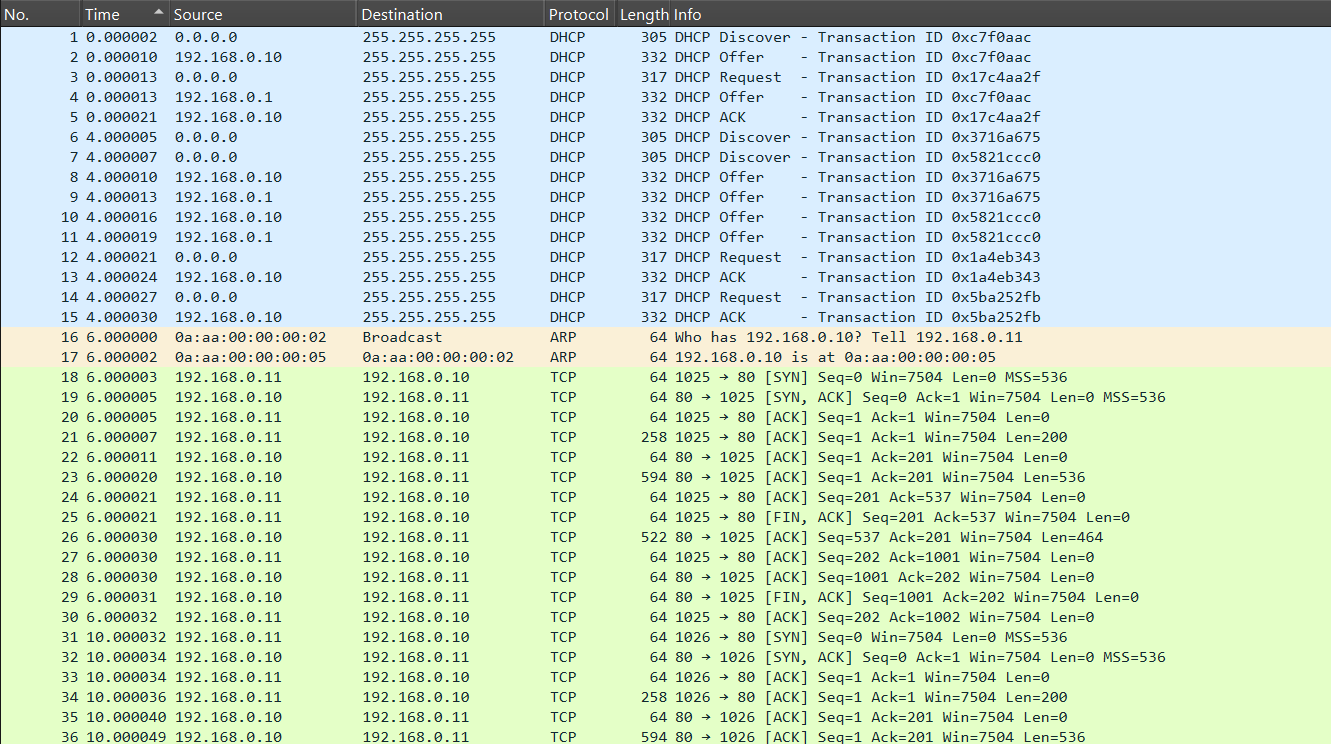
\includegraphics[width=135mm, scale=0.75]{imaxes/captura_ejer1_1.png}
    \caption{Tráfico DHCP entre host[0] y los servidores}
    \label{fig:captura_host0}
\end{figure}

Como podemos observar, el host[0] empieza haciendo un DHCP Discover para descubrir un servidor DHCP disponible. 
A continuación, el servidor local es el primero en responder la solicitud con un paquete DHCP Offer con una dirección IP disponible. El cliente (host[0]),
responde a su solicitud para confirmar la asignación ofrecida por el servidor local. El router también envía el paquete DHCP Offer, pero al enviarlo más tarde,
el cliente lo ignora. Finalmente, el servidor local contesta con un ACK (estos procesos se repiten para todos los cliente, host[1] y host[2]).

Posteriormente, el cliente host[0] intenta hacer la conexión con el servidor local, para lo cual manda primero un broadcast ARP, para asi saber 
cual es la MAC de la máquina, con la IP que establece en la cabecera ARP. Después, el servidor contesta al broadcast ARP que mandó el cliente identificandose su mac, ya que la cabecera ARP incluye su IP.

Finalmente, la conexión sigue adelante con los mensajes de la capa Trasporte correspondientes para la comunicación, restableciendose cada 4 segundos esa conexion (esto ocurre ya que establecemos un idleInterval de 4 segundos).




\section{Ejercicio 1.2}

\subsection{¿Cuál de los servidores proporciona la IP a host[0]? ¿Sabe el otro servidor que host[0] no cogió la IP ofrecida
por él? ¿Cómo? (Muestra el contenido de los paquetes relevantes en Wireshark.)}
 \chapter{IPv6-SLAAC}
\label{chap:ipv6_slaac}

\section{Ejercicio 2.1}
\subsection{Muestra una captura del escenario en el momento inicial de la simulación en la que se vean todas las
direcciones MAC e IP. Utilizando la dirección IP de host[0] como ejemplo, explica cómo se construye, destacando
los campos y bits relevantes. Utiliza para explicarlo la notación IPv6 no abreviada (16 bytes:
xxxx:xxxx:xxxx:xxxx:xxxx:xxxx:xxxx:xxxx)}

\begin{figure}[!ht]
    \centering
    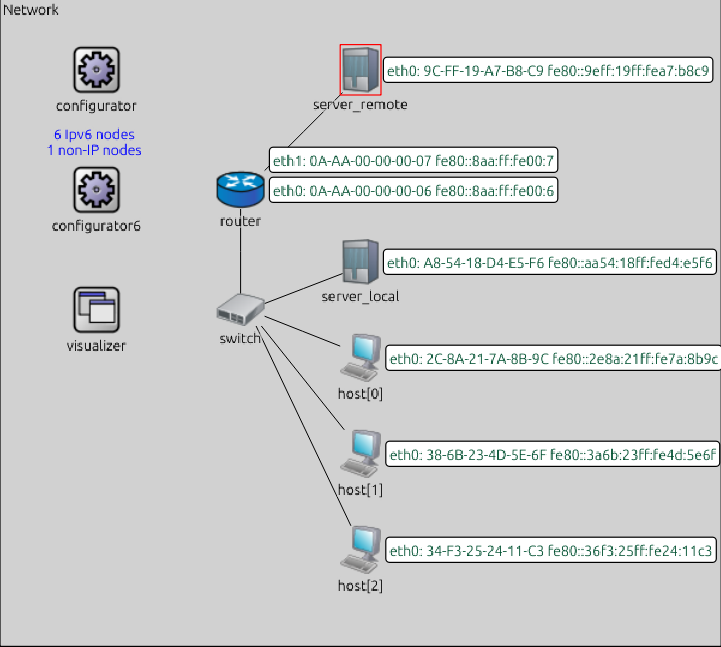
\includegraphics[width=135mm, scale=0.75]{imaxes/captura_ejer2_1.png}
    \caption{Escenario inicial dispositivos con IPv6}
    \label{fig:direccion_ipv6_host0}
\end{figure}

En el principio de la simulación, las direcciones que se muestran son direcciones unicast local de enlace. Estas son direcciones se generan automáticamente una vez que un dispositivo se conecta a una red. La estructura de este tipo de direcciones tienen como prefijo FE80::, no se enrutan y son únicas en ese enlace específico.

La segunda parte de la dirección se forma a partir de la dirección MAC del dispositivo. Para esto, fijamos el séptimo bit a 1 e insertamos 0XFFFE entre las dos mitades de la dirección MAC del dispositivo. 

Como ejemplo, vamos a ver la dirección unicast local de enlace que genera el dispositivo host[0]. Como vemos en la imagen \ref{fig:direccion_ipv6_host0}, su dirección está formada por el prefijo FE80:: y, después, 2E8A:21FF:FE7A:8B9C. Esa segunda parte, como se explicó antes, se forma a partir de su dirección MAC (2C-8A-21-7A-8B-9C). Como se puede observar, en los primeros 2 bytes de la dirección unicast local de enlace (2E8A), si lo comparamos con su dirección MAC, el segundo carácter se convierte en una E, ya que tenemos que añadir un uno en el séptimo bit (La letra C hexadecimal, que en binario es 1100, como su tercer bit corresponde al séptimo bit de la dirección unicast, pasa a ser 1 por lo que se convierte en E -> 1110). Llegados a este punto, tras el primer cambio, tenemos la siguiente estructura -> FE80::2E80:21.

Como se explicó anteriormente, una vez hecho el primer cambio, ahora añadimos 0XFFFE  y posteriormente los últimos 3 bytes de la dirección MAC, por lo que queda como dirección final unicast local de enlace\\ FE80::2E8A:21FF:FE7A:8B9C.


\section{Ejercicio 2.2}\label{chap:ejer22}
\subsection{Asigna al host[2] la misma dirección MAC que al host[0] y arranca la simulación. ¿Qué error ocurre antes de
que haya transcurrido el primer segundo de simulación? Muestra una captura del error que aparece. ¿Qué
paquete (tipo, origen y destino) provoca el error? ¿Por qué?}

\begin{figure}[!ht]
    \centering
    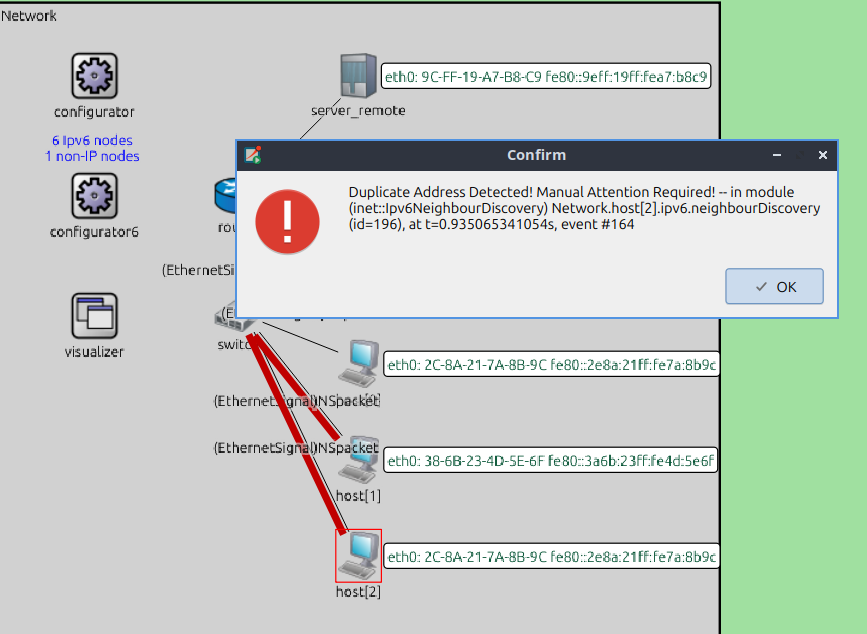
\includegraphics[width=135mm, scale=0.75]{imaxes/captura_ejer2_2.png}
    \caption{Fallo en la red con MAC host[2] igual a la de host[0]}
    \label{fig:fallo_ipv6_host2}
\end{figure}

Tal y como se muestra en la imagen \ref{fig:fallo_ipv6_host2}, hay un fallo de direcciones duplicadas cuando el host[2] intenta asignarse una dirección IPv6. 

El paquete en concreto que provoca el error es de tipo ICMPv6 con mensaje NS (Neighbor Solicitation), donde el origen de momento es el host[2] (En ese momento sin ninguna dirección) y como destino una dirección multicast. Este error ocurre porque el host[2], cuando crea su dirección, le comunica a sus vecinos de la red (DAD) cómo es su dirección.Entonces, se encuentra que el host[0] tiene la misma dirección IPv6 que él se asignó, por lo que ocurre un conflicto de IPs.

\section{Ejercicio 2.3}
\subsection{Cambia la MAC del host[2] de manera que coincida con la de host[0] en los últimos 3 bytes y difiera en los 3
primeros bytes (mantén esta MAC para el resto de las cuestiones). Asigna a serverremote la misma MAC que a
host[0]. ¿Vuelve a ocurrir el error de dirección duplicada con serverremote y host[0]? ¿Por qué?}

En este caso, al poner la misma MAC al host[0] y al server remote no produce ningún error porque son dispositivos que están en diferentes redes. 
El conflicto que sucedía en el ejercicio \ref{chap:ejer22} sucede porque los dos dispositivos estaban en la misma red, por lo que salta el error de 
direcciones duplicadas. Esto ocurre igual que en IPv4 con las IPs privadas: En la misma red no puede haber dos IPs iguales, pero si hay dos redes diferentes, puede coincidir una IP privada de un dispositivo que está en la red1 con la IP de otro dispositivo que esté en la red2.

\section{Ejercicio 2.4}
\subsection{¿Cuánto tiempo transcurre desde el principio de la simulación hasta que el host[0] su IP link-local definitiva
(i.e., fin de DAD)? Muestra la tabla de interfaces del nodo host[0] en la que se vea su estado antes y después del
DAD timeout y explica qué cambia. (Nota: Qtenv muestra toda la información de cada interfaz en una línea;
para verla correctamente copia el contenido con botón derecho → Copy Value y pégalo en la memoria como
texto, en lugar de usar capturas de pantalla.)}

Al comienzo de la simulación, host[0] comienza con su tabla de interfaces compuesta por la dirección de loopback en lo0 y su dirección IPv6 Link-Local en la interfaz eth0, producto de añadir al prefijo FF80:: el resultado de aplicar el proceso EUI-64 sobre su MAC. Esta última, como se aprecia en \ref{fig:InterfaceTableInicial}, está en estado \textit{tentative} hasta que el proceso de DAD inicial termine y se confirme que puede tomar esa dirección. \\
El timeout del DAD, que comenzó con el envío del paquete de Neighbor Solicitation en el t = 0.93 ( Ver \ref{fig:paquetes_IPv6_host0} ), finaliza en t=2.86, como se puede ver en \ref{fig:DAD_host0}. \\
De esta forma, la tabla de interfaces después de ese momento, \ref{fig:InterfaceTablePostDAD}, cambia ligeramente, desapareciendo el \textit{tentative} de la dirección. Esto se debe a que ningún vecino a contestado a su mensaje de NS en la red local, por lo que averigua que su dirección IP está libre y puede tomarla de forma definitiva.

\begin{figure}[H]
    \centering
    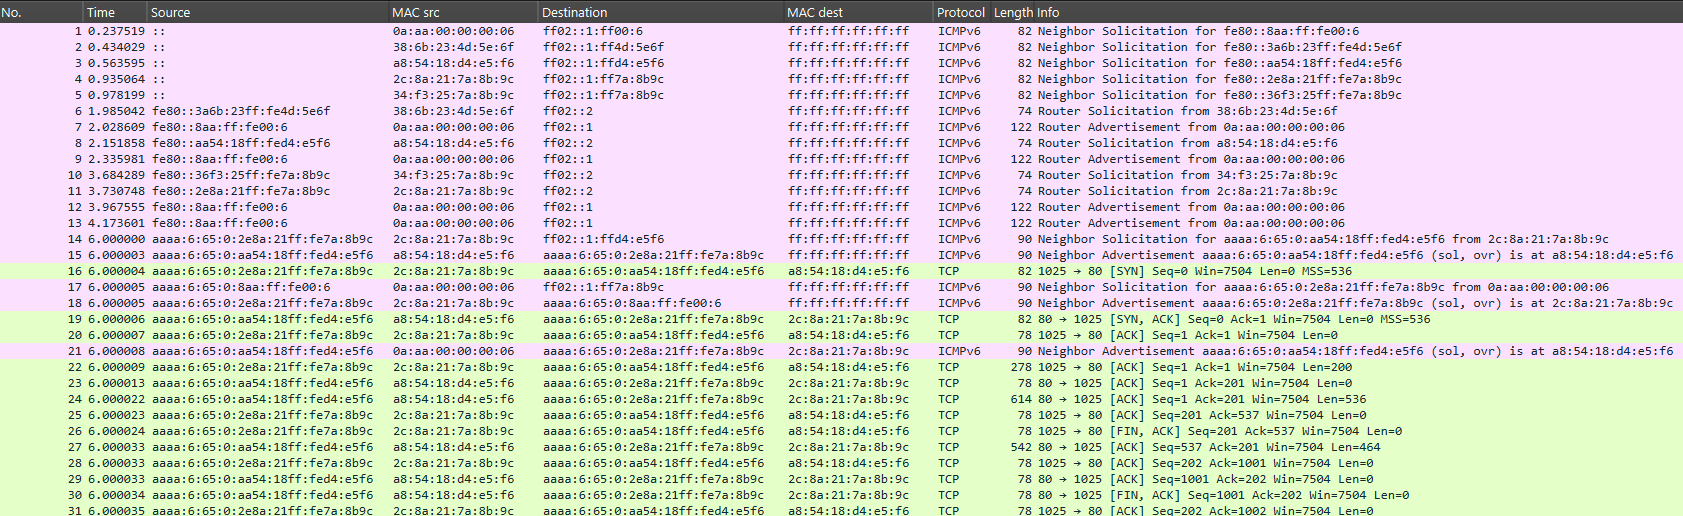
\includegraphics[width=135mm, scale=0.75]{imaxes/ejercicio2_4_1.png}
    \caption{Captura de paquetes entrantes y salientes de host[0]}
    \label{fig:paquetes_IPv6_host0}
\end{figure}

\begin{figure}[H]
    \centering
    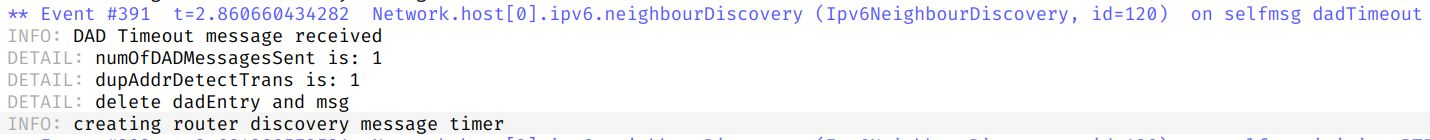
\includegraphics[width=135mm, scale=0.75]{imaxes/ejercicio2_4_2.png}
    \caption{Mensaje de fin de DAD para host[0]}
    \label{fig:DAD_host0}
\end{figure}

\begin{figure}[H]
    \centering
    \begin{lstlisting}
    lo0 ID:100 MTU:4470 UP LOOPBACK CARRIER macAddr:n/a Ipv6:{
        Addrs:::1(loopback)  expiryTime: inf prefExpiryTime: inf
        Node: dupAddrDetectTrans=1 reachableTime=36.455680949148
    }
    eth0 ID:101 MTU:1500 UP BROADCAST CARRIER MULTICAST macAddr:2C-8A-21-7A-8B-9C Ipv6:{
        Addrs:fe80::2e8a:21ff:fe7a:8b9c(link tent)  expiryTime: inf prefExpiryTime: inf
        mcastgrps:ff02::1 	Node: dupAddrDetectTrans=1 reachableTime=40.327972322702
    }
    \end{lstlisting}
    \caption{Tabla de interfaces de host[0] en t=0}
    \label{fig:InterfaceTableInicial}
\end{figure}

\begin{figure}[H]
    \centering
    \begin{lstlisting}
    lo0 ID:100 MTU:4470 UP LOOPBACK CARRIER macAddr:n/a Ipv6:{
	    Addrs:::1(loopback)  expiryTime: inf prefExpiryTime: inf
 	    Node: dupAddrDetectTrans=1 reachableTime=36.455680949148
   }

   eth0 ID:101 MTU:1500 UP BROADCAST CARRIER MULTICAST macAddr:2C-8A-21-7A-8B-9C Ipv6:{
	Addrs:fe80::2e8a:21ff:fe7a:8b9c(link)  expiryTime: inf prefExpiryTime: inf
	mcastgrps:ff02::1 	Node: dupAddrDetectTrans=1 reachableTime=40.327972322702
   }
    \end{lstlisting}
    \caption{Tabla de interfaces de host[0] en t=3}
    \label{fig:InterfaceTablePostDAD}
\end{figure}

\section{Ejercicio 2.5}
\subsection{¿En qué instante de la simulación obtienen los equipos sus direcciones IP globales? ¿Cómo obtienen esta
última? Muestra la tabla de interfaces de nodo host[0] en la que se vea su estado antes y después de obtener la
dirección global y explica qué cambia.}

Respecto a la captura de paquetes de la simulación realizada anteriormente ( Ver \ref{fig:paquetes_IPv6_host0} ), los equipos obtienen sus direcciones IP globales tras recibir un paquete de Router Advertisement. Como el primero en enviar un Router Solicitation es host[1] (Paquete número 6), es también el primero (Y único) que puede procesar el RA siguiente, obteniendo su dirección global en t=2.02. Después, ocurre lo mismo con server\_local, que obtiene su dirección en t=2.33, y con server\_remote, que la obtiene en t=2.72 (No se ve en \ref{fig:paquetes_IPv6_host0} porque server\_remote está en otra red). Finalmente, y como se observa parcialmente en \ref{fig:global_host0}, host[0] y host[2] obtienen la dirección global en t=2.72. Ambos la obtienen casi a la vez porque ambos emiten el paquete de Router Solicitation casi a la vez, de forma que, aunque el router devuelve dos paquetes RA, ambos obtienen la dirección global ya al recibir el primero. \\
Como se ha explicado en parte anteriormente, el proceso de obtener la dirección global comienza con un mensaje Router Solicitation del equipo al router correspondiente, enviado a la dirección multicast del grupo de los routers en el enlace local (FF02:02). En respuesta, el router responde un Router Advertisement en el que se anuncia junto con el prefijo global de la red correspondiente, que es con el que los nodos formarán su dirección global, a la dirección multicast de los nodos de la LAN (FF02::01). Los equipos que ya hayan enviado un paquete de RS pueden procesarlo, mientras que los que no lo hayan enviado o ya tengan una dirección global establecida, no. \\
Ahora, observando la tabla de interfaces de host[0] en \ref{fig:InterfaceTablePostGlobal}, observamos que una nueva dirección ha aparecido en la interfaz eth0, con la especificación \textit{global}, que se ha formado uniendo el prefijo global del red proporcionado por el router y la dirección MAC del dispositivo tras aplicar el proceso EUI-64, y a la que se le establece un tiempo de caducidad tras el que el equipo deberá volver a enviar un RS al router continuar teniendo una dirección global. Esta dirección es la que permite al dispositivo identificarse de forma única en Internet.

\begin{figure}[H]
    \centering
    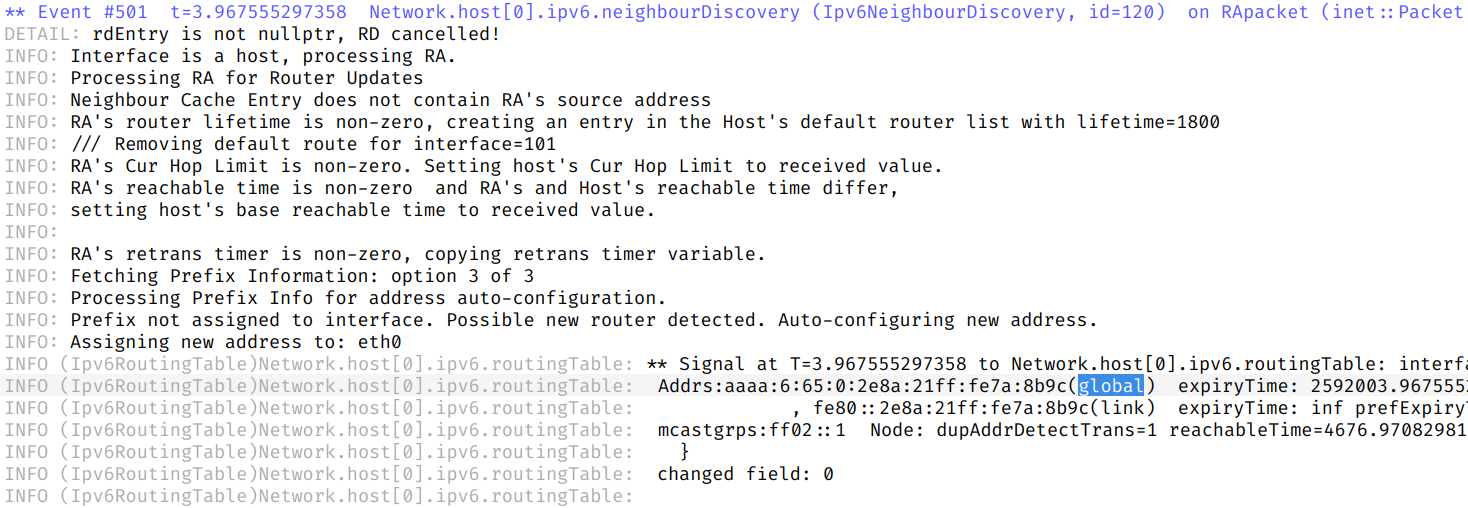
\includegraphics[width=135mm, scale=0.75]{imaxes/ejercicio2_5_1.png}
    \caption{Evento de obtención de dirección global para host[0]}
    \label{fig:global_host0}
\end{figure}

\begin{figure}[H]
    \centering
    \begin{lstlisting}
        lo0 ID:100 MTU:4470 UP LOOPBACK CARRIER macAddr:n/a Ipv6:{
            Addrs:::1(loopback)  expiryTime: inf prefExpiryTime: inf
            Node: dupAddrDetectTrans=1 reachableTime=36.455680949148
        }
        eth0 ID:101 MTU:1500 UP BROADCAST CARRIER MULTICAST macAddr:2C-8A-21-7A-8B-9C Ipv6:{
            Addrs:fe80::2e8a:21ff:fe7a:8b9c(link)  expiryTime: inf prefExpiryTime: inf
            mcastgrps:ff02::1 	Node: dupAddrDetectTrans=1 reachableTime=40.327972322702
        }
    \end{lstlisting}
    \caption{Tabla de interfaces de host[0] en t=3}
    \label{fig:InterfaceTablePostLocal}
\end{figure}

\begin{figure}[H]
    \centering
    \begin{lstlisting}
        lo0 ID:100 MTU:4470 UP LOOPBACK CARRIER macAddr:n/a Ipv6:{
            Addrs:::1(loopback)  expiryTime: inf prefExpiryTime: inf
                Node: dupAddrDetectTrans=1 reachableTime=36.455680949148
        }
        eth0 ID:101 MTU:1500 UP BROADCAST CARRIER MULTICAST macAddr:2C-8A-21-7A-8B-9C Ipv6:{
            Addrs:aaaa:6:65:0:2e8a:21ff:fe7a:8b9c(global)  expiryTime: 2592003.967555297358 prefExpiryTime: 604803.967555297358, 	
            fe80::2e8a:21ff:fe7a:8b9c(link)  expiryTime: inf prefExpiryTime: inf
            mcastgrps:ff02::1 	Node: dupAddrDetectTrans=1 reachableTime=4609.905032347888
        }
    \end{lstlisting}
    \caption{Tabla de interfaces de host[0] en t=4}
    \label{fig:InterfaceTablePostGlobal}
\end{figure}

\section{Ejercicio 2.6}
\subsection{Explica cómo se construye la IP global usando el nodo host[0] como ejemplo, de nuevo usando la notación
IPv6 no abreviada}

Una vez que el equipo manda un mensaje ICMPv6 con mensaje NS (Neighbor Solicitation) y no ocurre ningún fallo (No hay conflicto de IPs), procede a mandar un paquete ICMPv6 con mensaje RS (Router Solicitation), para que el router le asigne una IPv6 global (Este tipo de IPs ya son enrutables y únicas a nivel global). El router contesta con un paquete ICMPv6 con mensaje RA (Router Advertisement) indicando el prefijo global de red (Los primeros 64 bits de la dirección de la red al que está conectada host[0], en este caso AAAA:0006:0065:0000). Una vez que el host[0] obtiene el prefijo de la red, construye su IPv6 global substituyendo el prefijo de red del enlace local por la de la red, quedando su dirección como: AAAA:0006:0065:0000:2E8A:21FF:FE7A:8B9C. Esto se puede ver en la imagen \ref{fig:ip_global_host0}.

\begin{figure}[H]
    \centering
    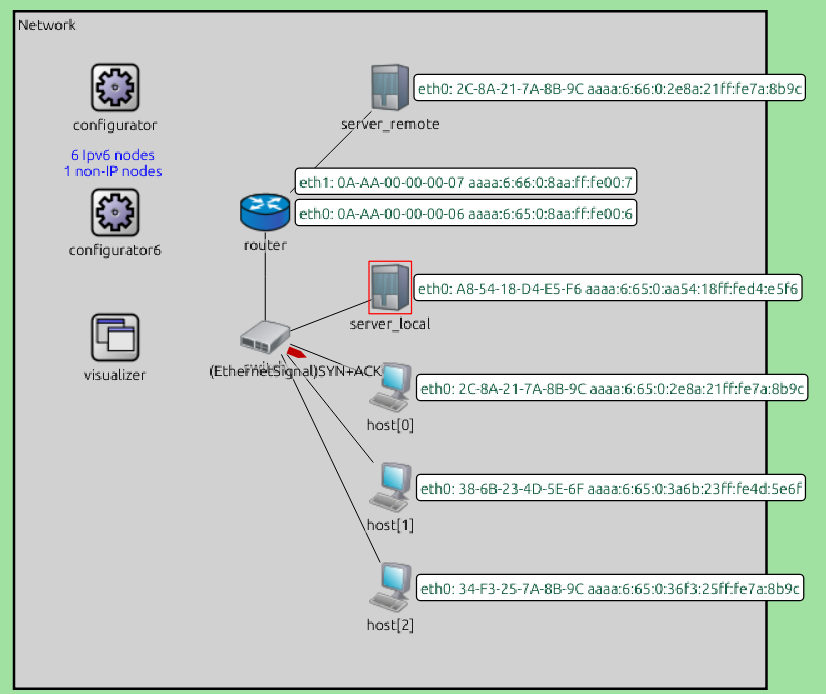
\includegraphics[width=135mm, scale=0.75]{imaxes/captura_ejer2_6.png}
    \caption{Foto red con direcciones IPv6 globales asignadas}
    \label{fig:ip_global_host0}
\end{figure}

\section{Ejercicio 2.7}
\subsection{Configura host[0] para que se conecte al servidor server remote usando su dirección fe80::x:x:x:x:
(asegúrate de que la dirección MAC de server remote es única). ¿Qué ocurre? Repite lo mismo para
server local. ¿Qué ocurre?}

Para realizar este ejercicio, se aplicaron los cambios descritos en la figura \ref{fig:conf_linklocalTCP} sobre la TcpBasicClientApplication de host[0], de forma que se conectara a los servidores directamente a través de su dirección de enlace local.\\
En primer lugar, probamos la conexión a server\_remote. Como se observa en la figura \ref{fig:conexion_serverRemote}, host[0] no recibe el ACK correspondiente a ninguno de sus paquetes de intento de conexión. La primera vez que intenta la conexión, no recibe respuesta, por lo que lo intenta de nuevo una y otra vez enviando TCP Retransmisions. Esto es debido a que server\_remote se encuentra en una LAN distinta a host[0], que intenta alcanzar su dirección de enlace local. Los routers en IPv6 no enrutan paquetes como lo hacen en IPv4 entre redes, por lo que la única forma que tendría host[0] de completar la conexión sería usando la dirección unicast global del servidor.\\
Por otra parte, descubrimos que al realizar la conexión con server\_local, ocurre lo mismo ( \ref{fig:conexion_serverLocal} ). Esto es debido a un comportamiento propio de INET, que limpia de la tabla de enrutamiento la dirección local de enlace ( \ref{fig:fallo1} ) que permite conectarse a otros dispositivos en el mismo segmento de red después de recibir el prefijo de red del router ( \ref{fig:fallo2} ). En la realidad, la conexión al servidor local sí debería realizarse con éxito, ya que está en la misma LAN que host[0] y debería poder descubrirlo en el proceso de Neighbor Discovery.

\begin{figure}[H]
    \centering
    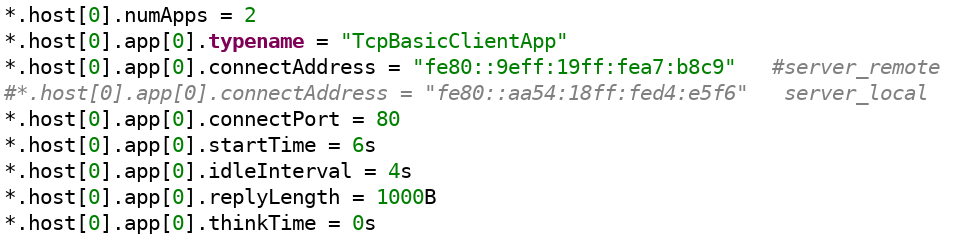
\includegraphics[width=135mm, scale=0.75]{imaxes/ejercicio2_7_1.png}
    \caption{Configuración establecida para este ejercicio}
    \label{fig:conf_linklocalTCP}
\end{figure}

\begin{figure}[H]
    \centering
    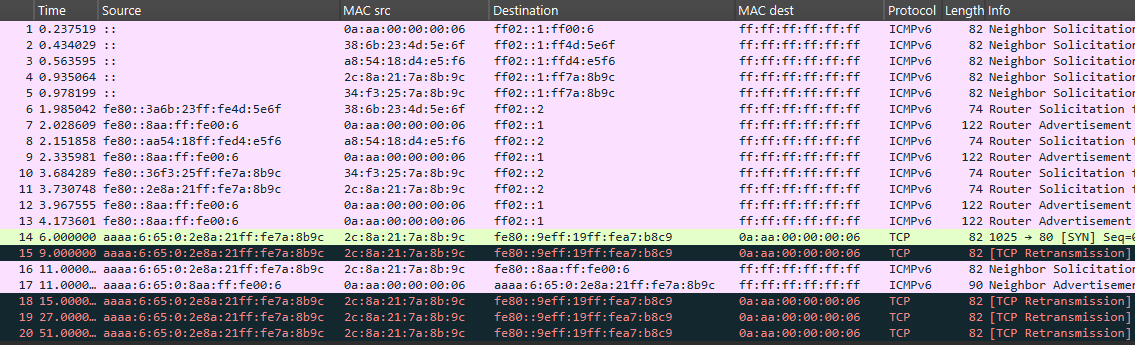
\includegraphics[width=135mm, scale=0.75]{imaxes/ejercicio2_7_3.png}
    \caption{Captura de paquetes en la conexión host[0] a server\_remote}
    \label{fig:conexion_serverRemote}
\end{figure}

\begin{figure}[H]
    \centering
    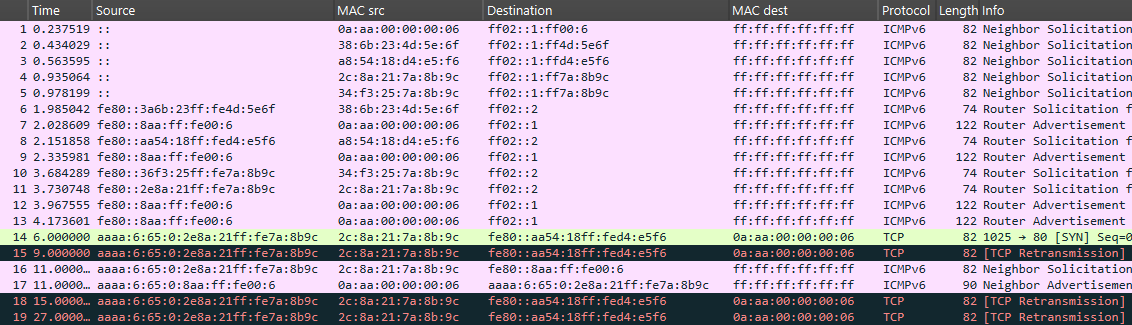
\includegraphics[width=135mm, scale=0.75]{imaxes/ejercicio2_7_2.png}
    \caption{Captura de paquetes en la conexión host[0] a server\_local}
    \label{fig:conexion_serverLocal}
\end{figure}

\begin{figure}[H]
    \centering
    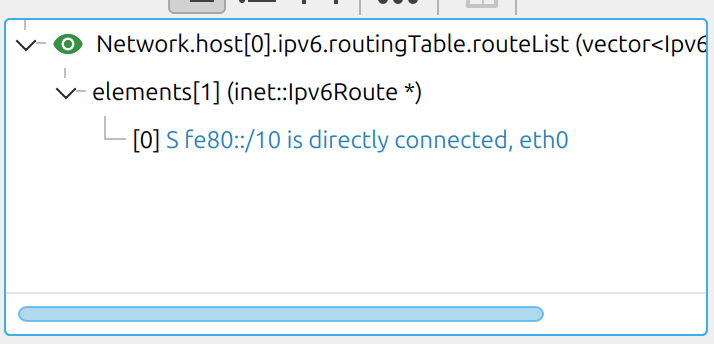
\includegraphics[width=65mm, scale=0.75]{imaxes/fallo1.png}
    \caption{Routing table de host[0] al inicio de la simulación}
    \label{fig:fallo1}
\end{figure}

\begin{figure}[H]
    \centering
    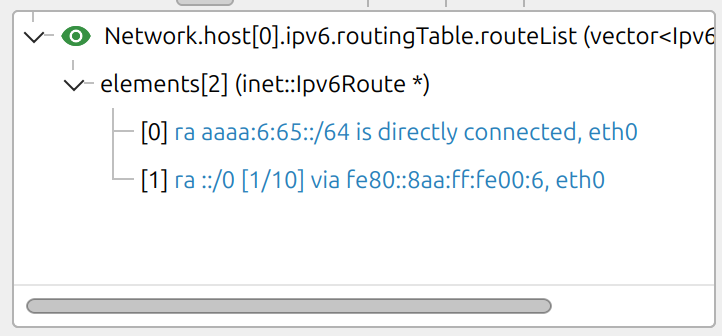
\includegraphics[width=65mm, scale=0.75]{imaxes/fallo2.png}
    \caption{Routing table de host[0] tras obtener la dirección unicast global}
    \label{fig:fallo2}
\end{figure}

 \chapter{IPv6-Multicast}
\label{chap:ipv6_multicast}

\section{Ejercicio 3.1}
\subsection{En los primeros 2 segundos de simulación se envían varios paquetes NS. Muestra una captura del tráfico de
paquetes en Wireshark en la que se vean las direcciones IP y MAC origen y destino de los NS enviados desde
cada uno de los nodos host[*]. (Nota: para mostrar las direcciones MAC añade dos nuevas columnas: Hw src
addr (unresolved) y Hw dest addr (unresolved). Colócalas a la derecha de las direcciones IP.) ¿De qué tipo son
las direcciones IP? ¿Cómo se construyen?}

\begin{figure}[H]
    \centering
    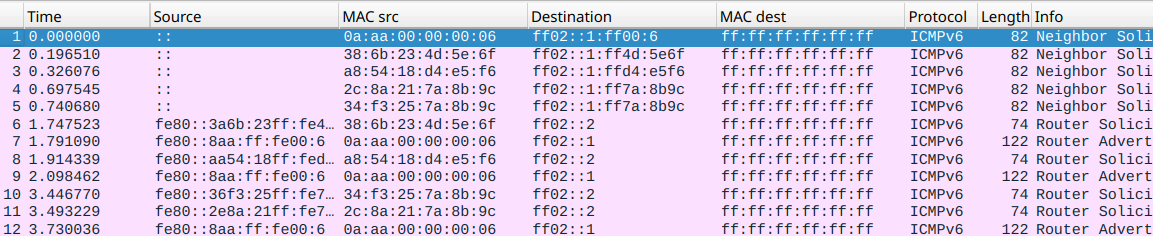
\includegraphics[width=135mm, scale=0.75]{imaxes/captura_ejer3_1.png}
    \caption{Captura MAC origen y destino host[0]}
    \label{fig:ip_mac_host0}
\end{figure}

Como las direcciones IPs de destino son multicast, en todos los hosts se ve la misma paquetería, por lo que solo subimos la captura de tráfico en el host[0].

Las direcciones, como hemos mencionado anteriormente, son multicast y se construyen con el prefijo multicast link-local (FF02::1, donde FF02 quiere decir que es tipo multicast, siendo el 2 un scope de local de enlace y el último 1 quiere decir todos los dispositivos. Si fuera un 2 serían todos los routers). Por último, tendríamos como sufijo, los 3 bytes menos significativos de la MAC del dispositivo de ese host precedido de FF.

Por ejemplo, en el primer caso tenemos como destino FF02::1:FF00:0006 donde F002::1 es, como explicamos antes, el prefijo multicast link-local y como sufijo FF00:0006, donde 000006 son los 3 últimos bytes de la MAC de la interfaz del router en ese enlace (0A:AA:00:00:00:06).

\section{Ejercicio 3.2}
\subsection{¿Coincide alguna de las direcciones IP destino de los diferentes paquetes NS? ¿Por qué? ¿Qué consecuencia
tiene esto?}

Coinciden las direcciones IP del host[0] y host[2], ya que los dos tienen los 3 últimos bytes de la MAC iguales por lo que la dirección multicast se construye de la misma forma.

Con respecto a las consecuencias que se puede tener al haber dos direcciones multicast iguales, no hay ninguna, ya que los mensajes ICMPv6 de tipo NS (Neighbor Solicitation) guardan en su cabecera la dirección unicast de destino, por lo que no se daría ningún conflicto (target address). Aunque no pase nada, lo normal es que las direcciones multicast de nodo solicitado (FF02::1) sean únicas.


\section{Ejercicio 3.3}
\subsection{¿Por qué se envían los NS a esas direcciones IP?}

Se envían ICMPv6 de tipo NS a esas direcciones ya que haciéndolo con direcciones multicast, se puede mandar un único paquete a uno o varios destinos, de esta forma optimizamos la comunicación y reducimos el tráfico de la red para que no se congestione por lo que aumenta la eficiencia. 


\section{Ejercicio 3.4}
\subsection{¿Qué direcciones MAC destino tienen los paquetes NS anteriores? ¿Cuáles deberían tener según lo visto en
clases de teoría? (Utiliza el paquete NS que sale desde host[1] como ejemplo y escribe los 6 bytes que debería
tener la dirección MAC en formato hexadecimal.)}

\begin{figure}[H]
    \centering
    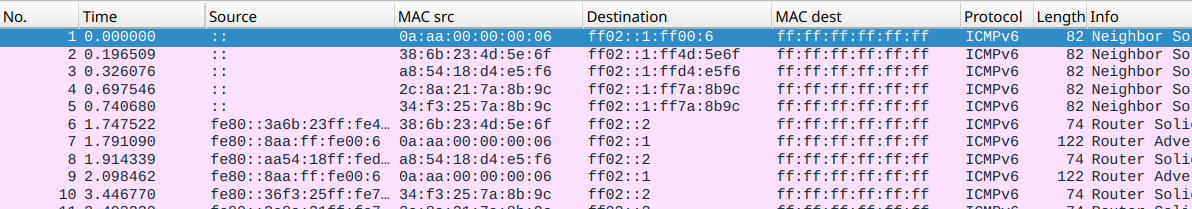
\includegraphics[width=135mm, scale=0.75]{imaxes/captura_ejer3_4.png}
    \caption{Captura MAC origen y destino paquetes NS en host[1]}
    \label{fig:ip_mac_host1}
\end{figure}

Como se puede observar en la imagen \ref{fig:ip_mac_host1}, todos los paquetes tienen como MAC destino FF:FF:FF:FF:FF:FF. Según se ha visto en la clase de teoría, las MAC tienen la estructura 33:33:FF como prefijo de la MAC y, después, los 3 últimos bytes son los 3 bytes menos significativos de la dirección multicast. En este caso, el destino es la dirección MAC broadcast, ya que Omnett no sabe como construir este tipo de direcciones MAC como se explica en la teoría, por eso todos los hosts reciben la misma paquetería. De la otra forma, cada uno recibiría su propia paquetería.

\section{Ejercicio 3.5}
\subsection{¿Qué consecuencia tiene esta diferencia con respecto a lo visto en clase de teoría?}

Resulta que las consecuencias de usar dirección MAC broadcast es que todo el mundo recibe paquetes que en realidad no tendrian que recibir por lo que se sobrecarga la red. Usando la direccion MAC que se especifica en la teoria, solamente se mandaría el paquete a ese host.

\section{Ejercicio 3.6} 
\subsection{Muestra las direcciones IP y MAC destino de los mensajes RS y RA que aparecen en torno al segundo 2 de
simulación. ¿De qué tipo son las direcciones IP?}

\begin{figure}[H]
    \centering
    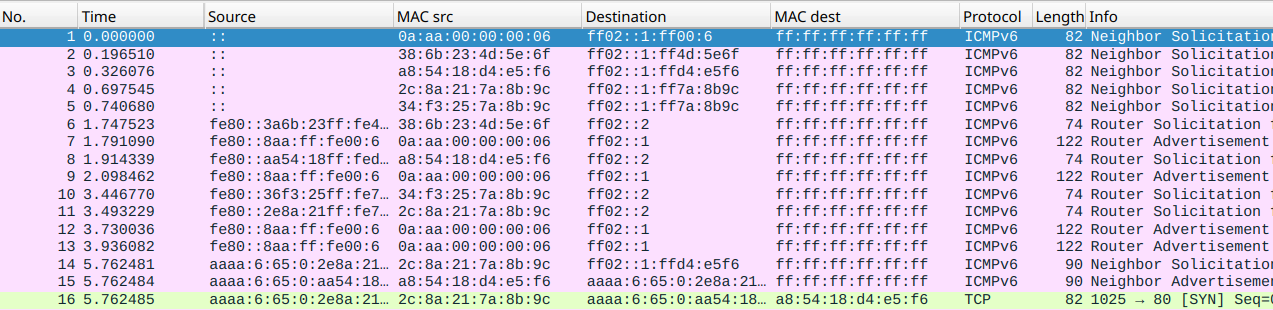
\includegraphics[width=135mm, scale=0.75]{imaxes/captura_ejer3_6.png}
    \caption{Captura paquetes RS y RA host[0]}
    \label{fig:rs_ra_h1}
\end{figure}

Como se puede observar en la imagen \ref{fig:rs_ra_h1}, en el caso de los paquetes ICPMv6 con mensaje RS tienen como dirección destino la direccion multicast FF02::2 y como MAC de destino, la dirección FF:FF:FF:FF:FF:FF. En este caso, las direcciones multicast son de este tipo ya que son direcciones a las que van dirigidos los paquetes a todos los routers de la misma red de en enlace para así optimizar el proceso de descubrimiento de routers y no malgastar ancho de banda.

En el caso de los paquetes ICMPv6 con mensaje RA, estos tienen como dirección destino la dirección multicast FF02::1 y como MAC de destino la dirección FF:FF:FF:FF:FF:FF. En este caso, la dirección multicast tiene esta estructra ya que va dirigido a todo dispositivo que está en el mismo enlace de red. 

\section{Ejercicio 3.7}
\subsection{¿Por qué el RA de respuesta a un RS no usa IP destino unicast?}

Este enfoque permite enviar la información de configuración a todos los dispositivos de la red sin necesidad de identificar la dirección específica de cada uno. Si se utilizara una dirección unicast, sería necesario conocer la dirección única de cada dispositivo, lo que resultaría poco práctico en redes grandes o cuando los dispositivos conectados pueden cambiar con frecuencia. Así, de esta forma, el tráfico no se sobrecarga y resultaría todo mas eficiente.

\section{Ejercicio 3.8}
\subsection{¿Qué direcciones MAC destino deberían tener los RS según lo visto en clases de teoría? ¿Y los RA?}

La MAC destino del paquete RS debería ser 33:33:00:00:00:02, asegurando que solo los routers reciban las solicitudes de descubrimiento de nodos, y los paquetes RA deberían tener como MAC destino 33:33:00:00:00:01, por lo que así sería captado por las interfaces Ethernet de todos los dispositivos IPv6 de esa misma red.

\section{Ejercicio 3.9}
\subsection{ Aproximadamente en t = 6 s el router envía dos NS. ¿De qué tipo son las direcciones IP destino de estos
paquetes? Explica cómo se construyen (notación IPv6 no abreviada).}

En IPv6, las direcciones de destino de los mensajes de Neighbor Solicitation son direcciones multicast de nodo solicitado. Estas direcciones se utilizan en el protocolo Neighbor Discovery para resolver la dirección MAC correspondiente a una dirección IPv6 de destino específica en la red local o para anunciar la presencia del emisor del paquete en el proceso de Duplicate Address Detection (El caso estudiado en este ejercicio es el especificado en primer lugar). Cada dirección unicast IPv6 tiene asociada una dirección multicast de nodo solicitado, las cuales, a su vez, se corresponden siempre con una direccion multicast Ethernet.\\
Las direcciones multicast de nodo solicitado se forman añadiendo tras el prefijo \\
FF02::1:FF00:0000/104 (ff02:0000:0000:0000:0000:0001:ffXX:XXXX) los 24 bits menos significativos de la dirección unicast correspondiente. \\
En nuestro caso, como se observa en el paquete 15 de la figura \ref{fig:ns_from_router_to_host0}, la dirección de destino es, siguiendo la notacioón IPv6 no abreviada, 
ff02:0000:0000:0000:0000:0001:ff7a:8b9c. De esta forma, el paquete será procesado solo por aquellos equipos cuya dirección unicast termine por 7a:8b9c, aunque sea enviado a todos los nodos en la red del destinatario.

\begin{figure}[H]
    \centering
    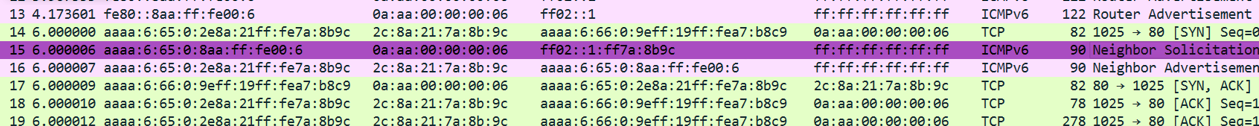
\includegraphics[width=135mm, scale=0.75]{imaxes/ejercicio3_9_1.png}
    \caption{Intercambio de paquetes en t=6 entre el router y host[0]}
    \label{fig:ns_from_router_to_host0}
\end{figure}

\section{Ejercicio 3.10}
\subsection{¿En qué equipos llega el segundo paquete NS enviado por el router al módulo ipv6? ¿Y al submódulo
ipv6.neighborDiscovery? ¿Por qué? (Nota: para ver el recorrido del paquete en el módulo ipv6, haz doble click en
el nodo deseado y luego en el módulo ipv6. Puedes mostrar varios nodos a la vez en diferentes ventanas con
botón derecho → Open Graphical View for ‘ipv6’ una vez dentro de ese nivel.)}

En primer lugar, cabe destacar que el segundo paquete NS al que nos referiremos en este ejercicio es el que aparece en la figura \ref{fig:ns_from_router_to_host0}, es decir, el enviado del router al switch de la LAN a la que está host[0] conectado. Esto se sabe, porque, como se aprecia en la figura \ref{fig:ns_logs}, el primer paquete (Evento 569) es enviado hacia el servidor remoto; mientras que el evento 605 refleja el envío de ese segundo paquete hacia la dirección multicast de nodo solicitado de host[0].\\
El paquete NS es primero enviado al switch, que, a su vez, lo reenvía a todos los hosts y a server\_local. Esto se debe a que INET no implementa correctamente direcciones MAC multicast, por lo que la dirección de nodo solicitado de destino equivale a la dirección broadcast de capa 2, ff:ff:ff:ff:ff:ff (Ver \ref{fig:ns_from_router_to_host0}). Podemos ver en detalle en las figuras \ref{fig:ns_ipv6_host0} y \ref{fig:ns_ipv6_host1}, que el paquete entra al módulo IPv6, tanto de host[0] como de host[1], que realmente no es el objetivo de esta transmisión (De igual forma ocurre en server\_local y host[2]).\\
Por otra parte, se puede ver en la comparación representada en la figura \ref{fig:ns_ipv6ND_host0host1} entre host[0] y host[1], el paquete solo pasa al módulo neighborDiscovery en el caso de host[0], ya que es previamente procesado en el módulo IPv6, donde sí puede leerse su dirección destino de nodo solicitado. Sin embargo, debido a que host[0] y host[2] tienen los últimos 3 bytes de su MAC, y por lo tanto, de su direccción multicast de nodo solicitado, idénticos, el paquete es recibido también en el módulo IPv6 de host[2] (Ver \ref{fig:ns_ipv6ND_host2}).\\
En resumen, el paquete NS alcanza el módulo IPv6 de host[0], host[1], host[2] y server\_local y el módulo neighborDiscovery de host[0] y host[2], únicamente. 

\begin{figure}[H]
    \centering
    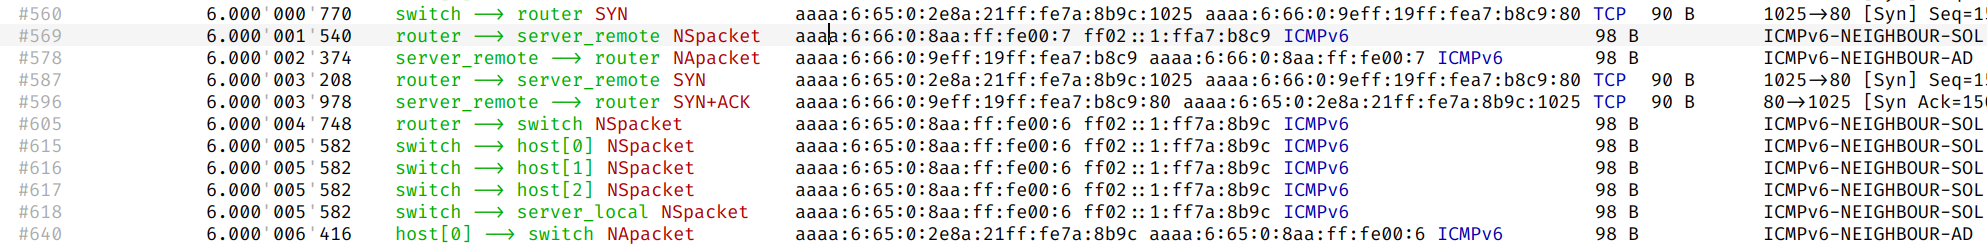
\includegraphics[width=135mm, scale=0.75]{imaxes/ejercicio3_10_1.png}
    \caption{Paquetes enviados por el router en t=6 (Captura de log)}
    \label{fig:ns_logs}
\end{figure}

\begin{figure}[H]
    \centering
    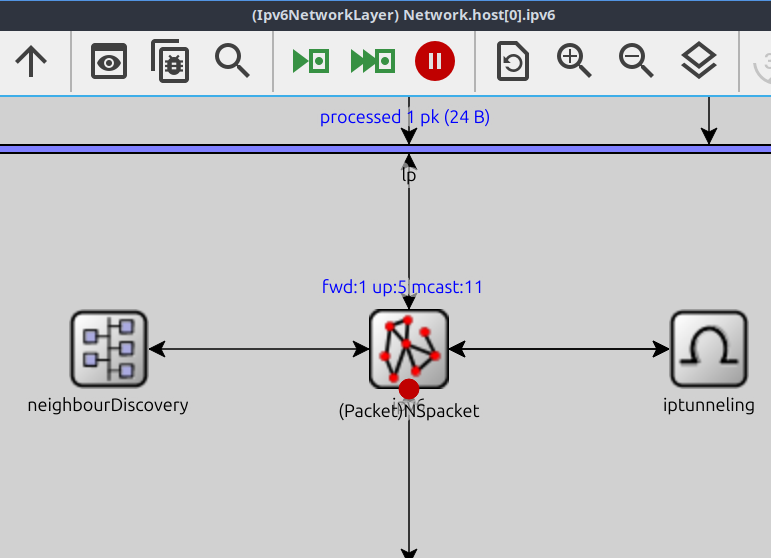
\includegraphics[width=135mm, scale=0.75]{imaxes/ejercicio3_10_2.png}
    \caption{Paquete de NS entrando al módulo IPv6 de host[0]}
    \label{fig:ns_ipv6_host0}
\end{figure}

\begin{figure}[H]
    \centering
    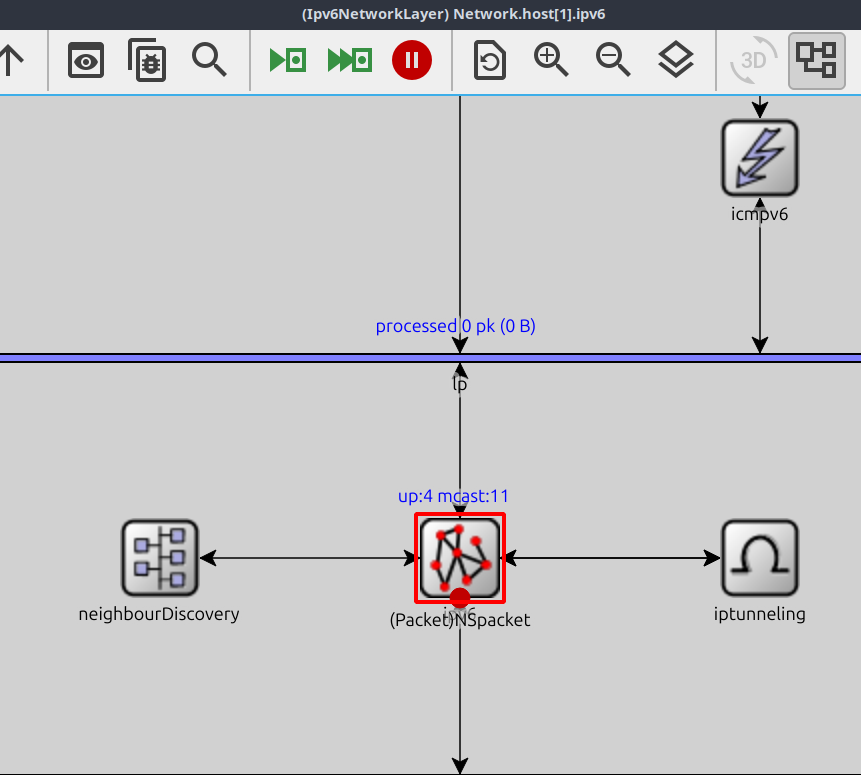
\includegraphics[width=135mm, scale=0.75]{imaxes/ejercicio3_10_3.png}
    \caption{Paquete de NS entrando al módulo IPv6 de host[1]}
    \label{fig:ns_ipv6_host1}
\end{figure}

\begin{figure}[H]
    \centering
    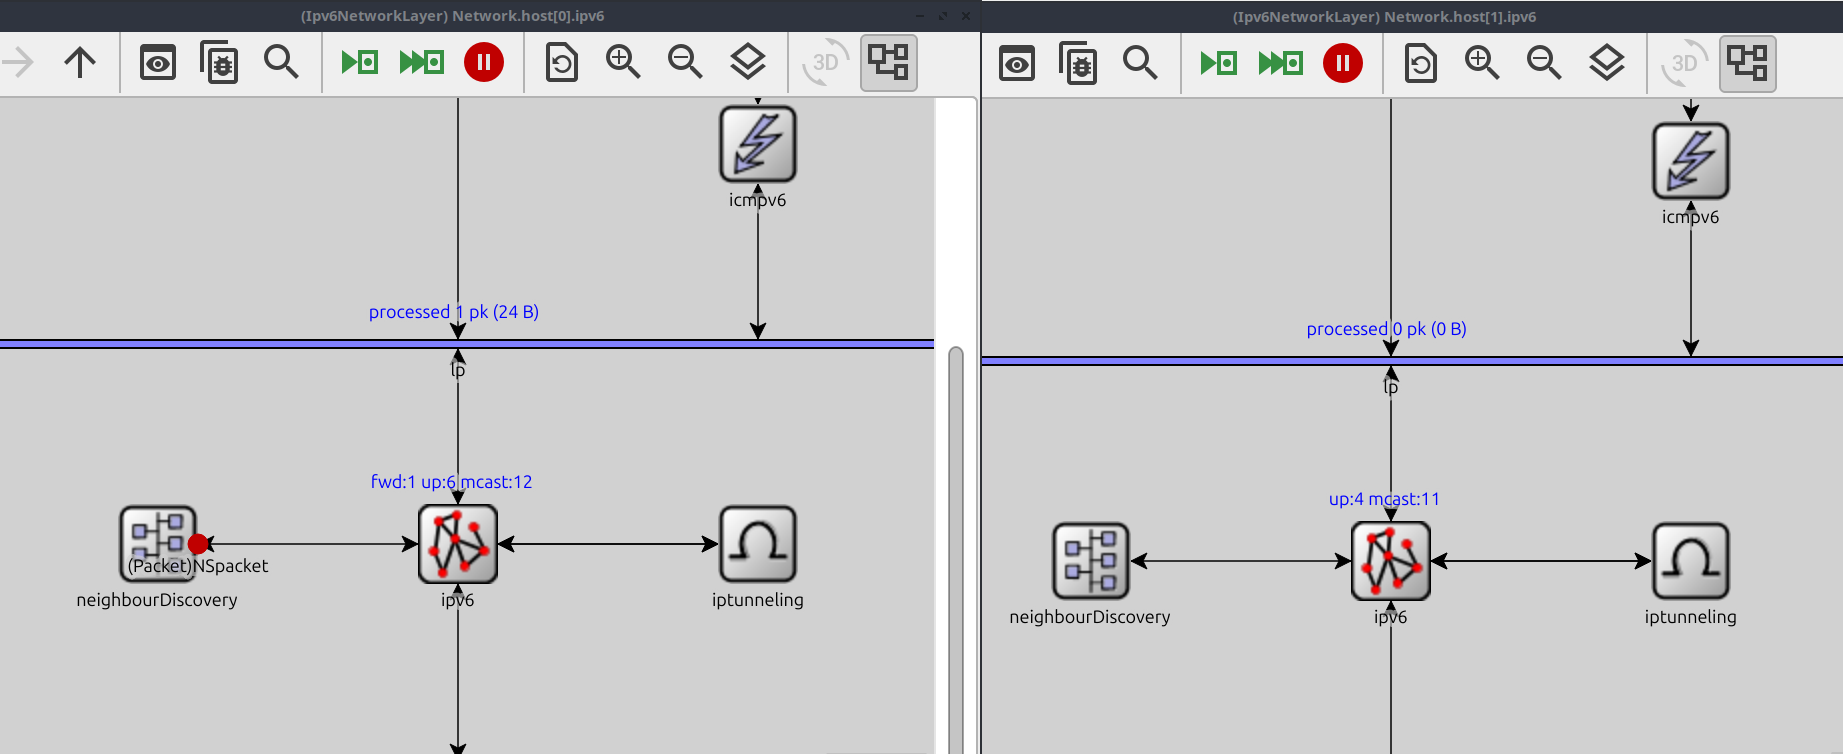
\includegraphics[width=135mm, scale=0.75]{imaxes/ejercicio3_10_4.png}
    \caption{Comparación entre host[0] y host[1] de paquetes entrantes al módulo neighborDiscovery}
    \label{fig:ns_ipv6ND_host0host1}
\end{figure}

\begin{figure}[H]
    \centering
    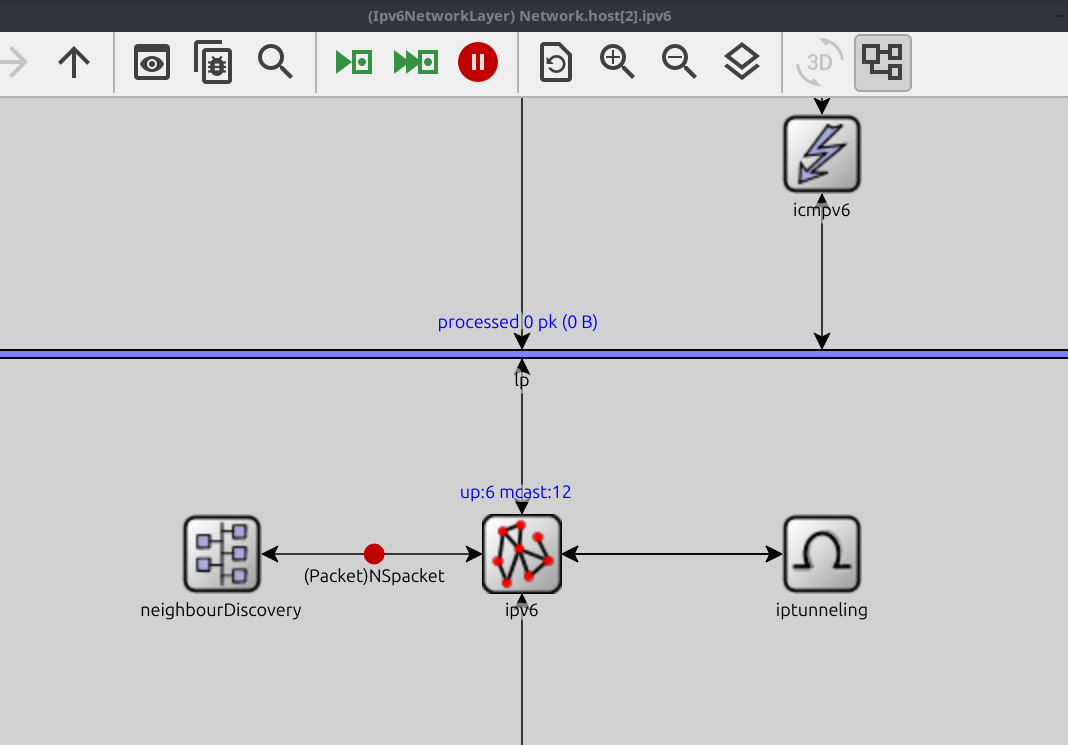
\includegraphics[width=135mm, scale=0.75]{imaxes/ejercicio3_10_5.png}
    \caption{Paquete de NS entrando al módulo neighborDiscovery en host[2]}
    \label{fig:ns_ipv6ND_host2}
\end{figure}

\section{Ejercicio 3.11}
\subsection{¿En qué equipos llegaría el mensaje al módulo ipv6 si INET implementase direcciones MAC multicast (33-
33-xx-xx-xx-xx)? ¿Por qué?}

Si INET implementase este tipo de direcciones, el mensaje llegaría al modulo IPv6 (Prefijo 33-33) de los equipos que tengan asignada la dirección MAC 33-33-xx-xx-xx-xx, siendo los últimos 32 bits iguales a los últimos 32 de la dirección multicast de nodo solicitado del equipo. O lo que es lo mismo, el prefijo FF seguido de los últimos 24 bits de la dirección unicast correspondiente a la de nodo solicitado. \\
Como la configuración actual asigna a host[0] y host[2] direcciones MACC que coinciden en los ultimos 3 bytes, el mensaje NS al que nos referimos, con destino 33-33-FF-7A-8B-9C, sería recibido por los módulos IPv6 de los equipos host[0] y host[2] únicamente y no a todos los equipos actualmente existentes en la LAN, como ocurre en la situación estudiada en el ejercicio anterior.
 %\chapter{Otras Gráficas}
\label{chap:sinqos}

\begin{figure}[!ht]
    \centering
    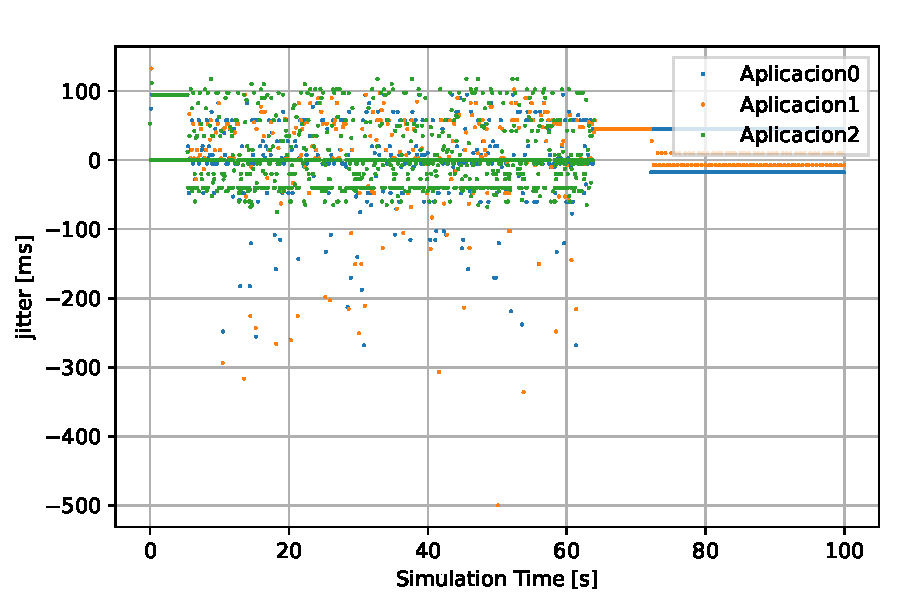
\includegraphics{graficas/sinQoS/jitter_SinQoS.pdf}
    \caption{Jitter a partir retardo extremo a extremo del router sin QoS}
    \label{fig:sinqos_jitter}
\end{figure}

\begin{figure}
    \centering
    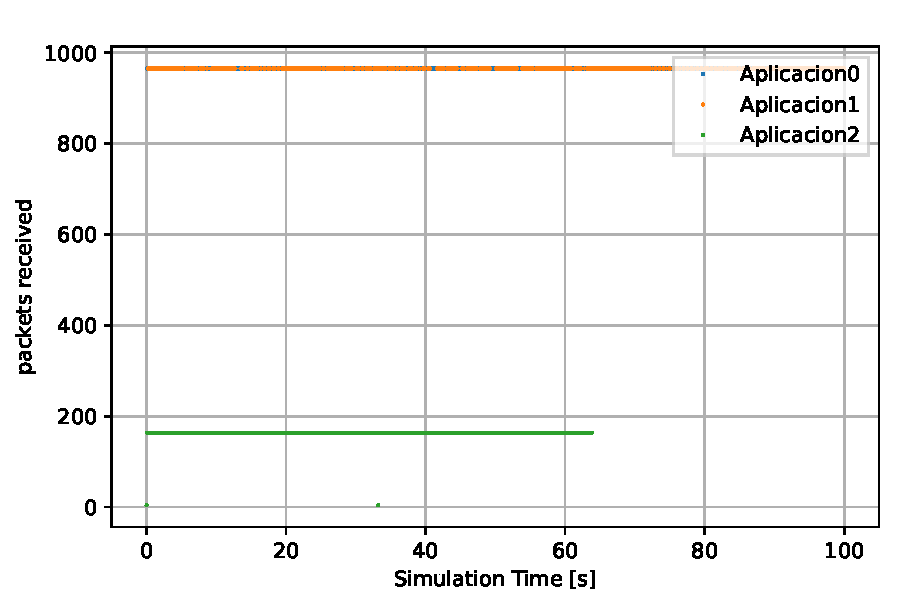
\includegraphics{graficas/sinQoS/packetsReceived_sinQoS.pdf}
    \caption{Paquetes recibidos en el servidor sin QoS}
    \label{fig:sinqos_pktreceived}
\end{figure}

\begin{figure}
    \centering
    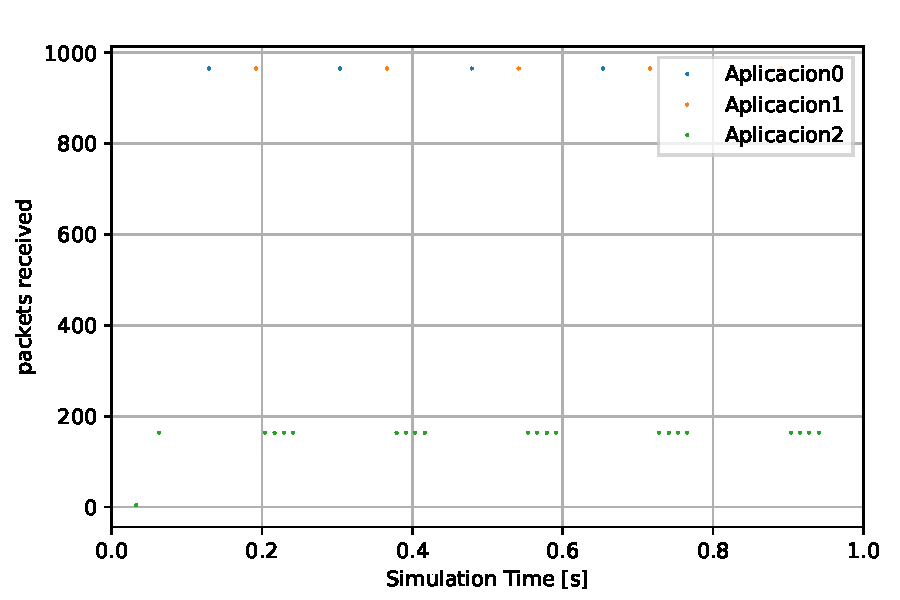
\includegraphics{graficas/sinQoS/packetsReceived_sinQoS_1.pdf}
    \caption{Paquetes recibidos en el servidor sin QoS intervalo 0-1}
    \label{fig:sinqos_pktreceived01}
\end{figure}

\begin{figure}
    \centering
    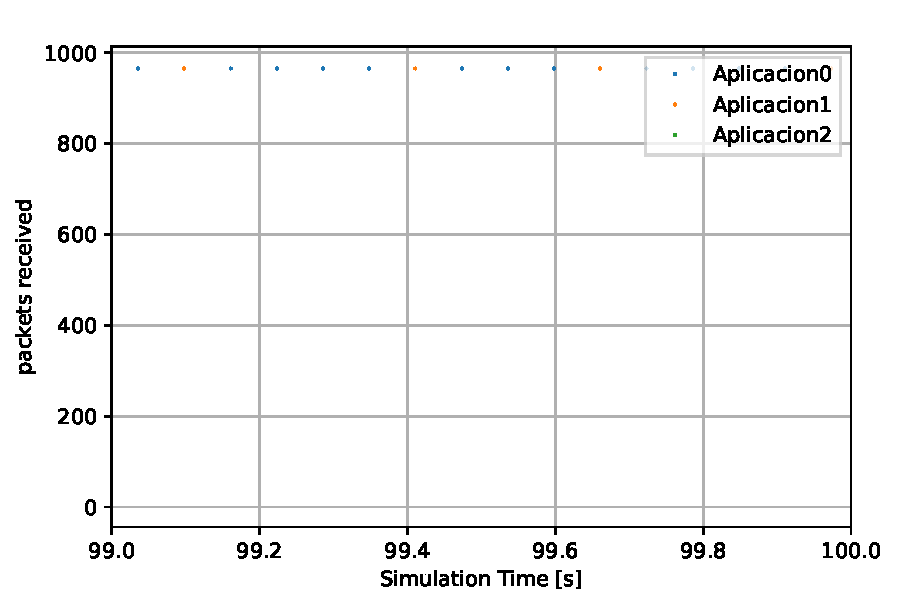
\includegraphics{graficas/sinQoS/packetsReceived_sinQoS_99.pdf}
    \caption{Paquetes recibidos en el servidor sin QoS intervalo 99-100}
    \label{fig:sinqos_pktreceived99100}
\end{figure}


\begin{figure}[!ht]
    \centering
    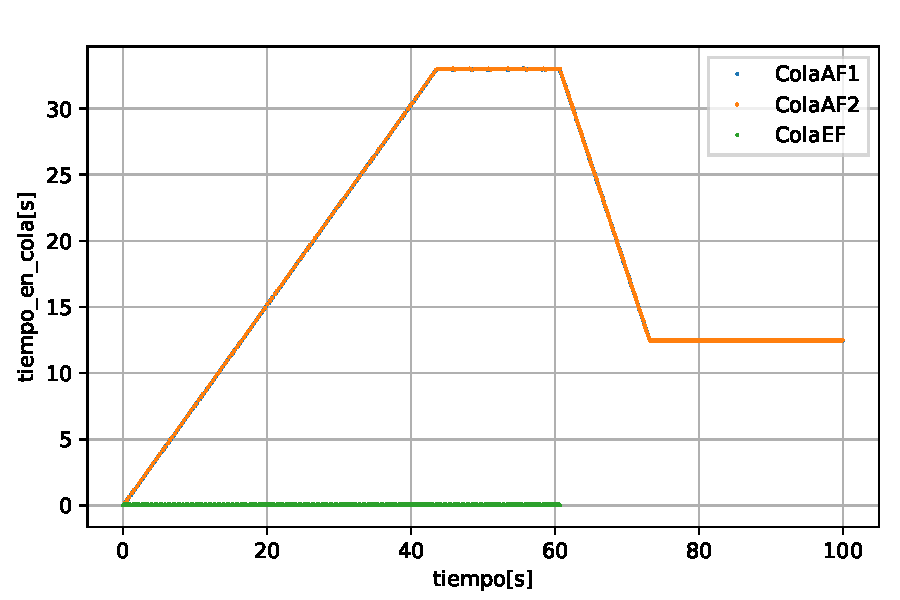
\includegraphics{graficas/DropTail/tiempo_en_cola_droptail.pdf}
    \caption{Tiempo encolado droptail}
    \label{fig:droptail_time}
\end{figure}

\begin{figure}
    \centering
    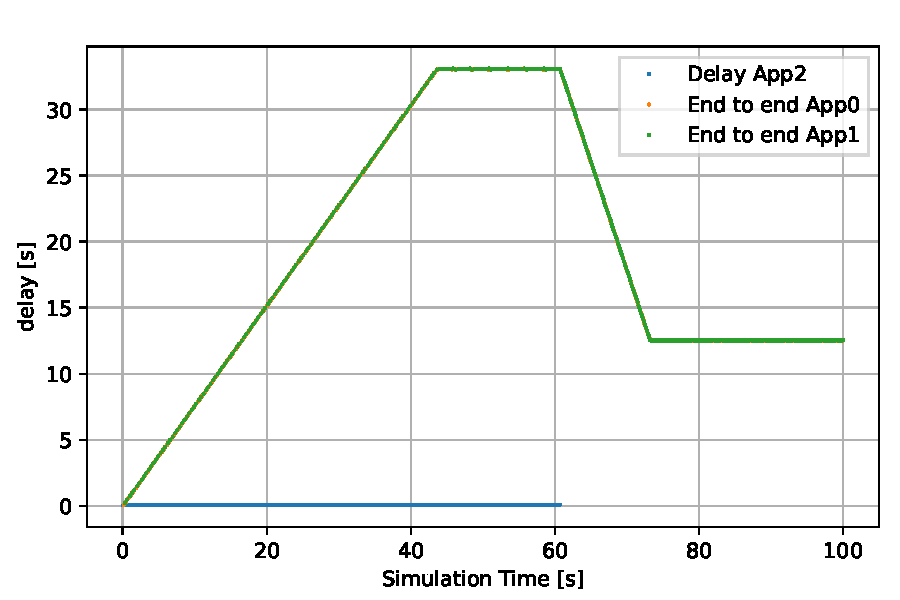
\includegraphics{graficas/DropTail/delay_DT.pdf}
    \caption{Delay extremo a extremo con droptail}
    \label{fig:sinqos_pktreceived99100}
\end{figure}

\begin{figure}
    \centering
    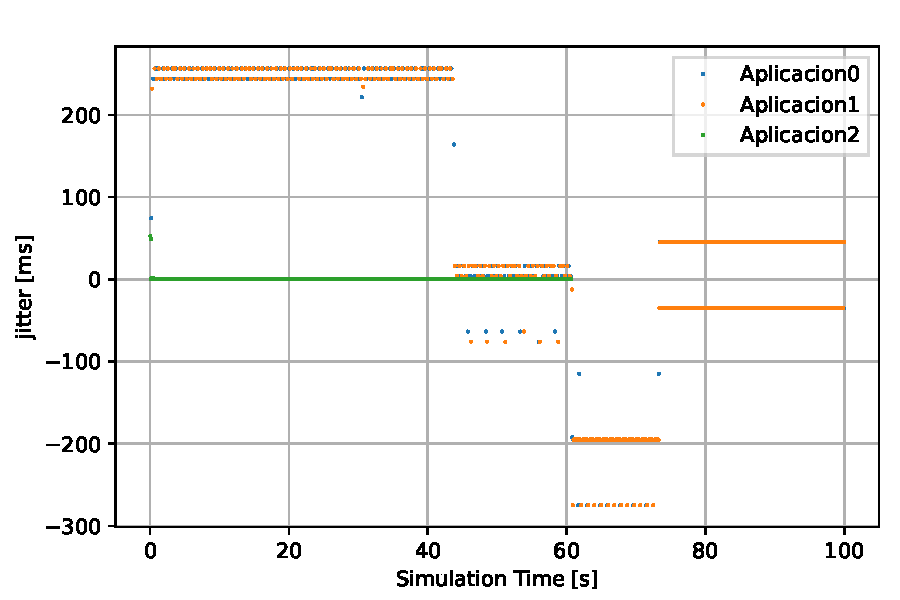
\includegraphics{graficas/DropTail/jitter_DT.pdf}
    \caption{Jitter a partir retardo extremo a extremo droptail}
    \label{fig:sinqos_pktreceived99100}
\end{figure}

\begin{figure}
    \centering
    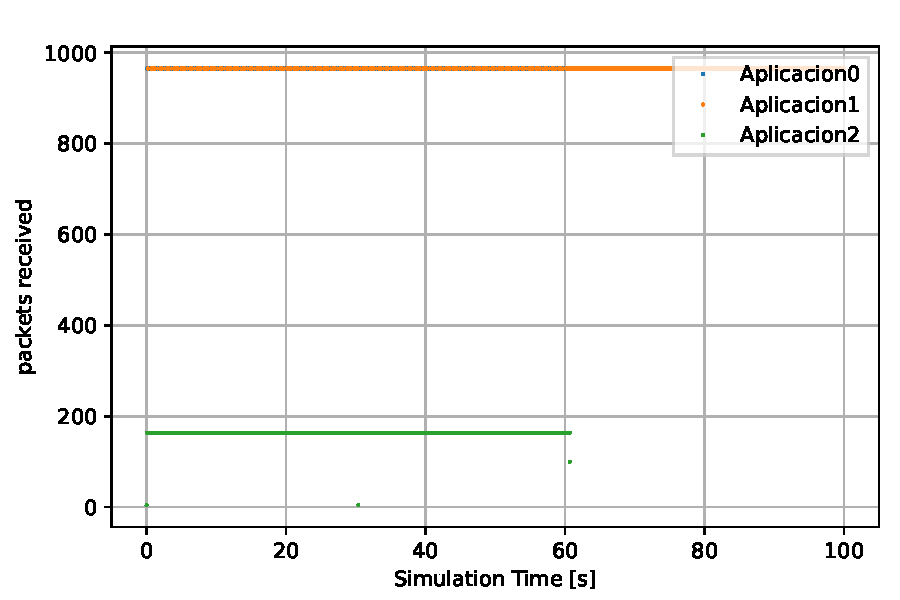
\includegraphics{graficas/DropTail/packetsReceived_DT.pdf}
    \caption{Paquetes recibidos en el servidor droptail}
    \label{fig:sinqos_pktreceived99100}
\end{figure}

\begin{figure}
    \centering
    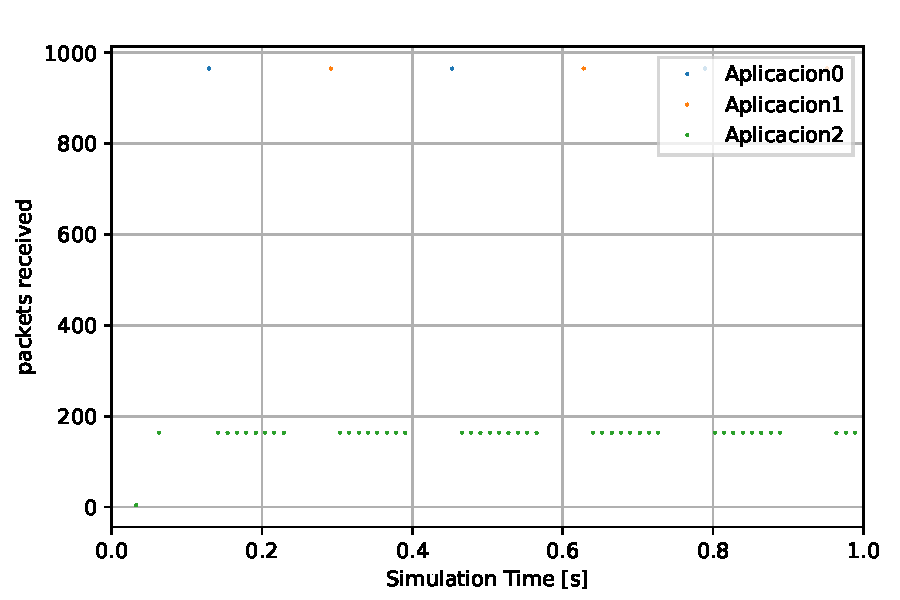
\includegraphics{graficas/DropTail/packetsReceived_DT_1.pdf}
    \caption{Paquetes recibidos en el sevidor droptail intervalo 0-1 }
    \label{fig:sinqos_pktreceived99100}
\end{figure}

\begin{figure}
    \centering
    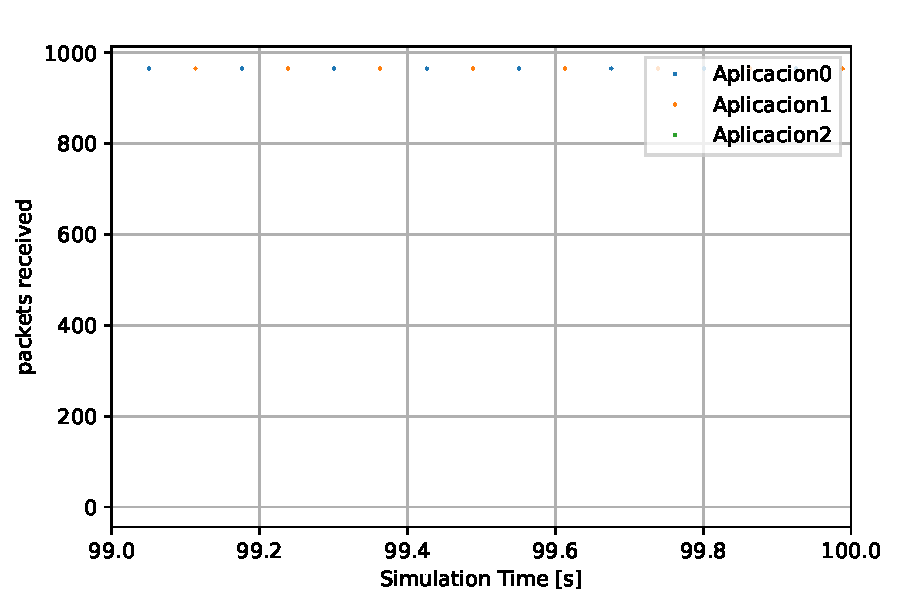
\includegraphics{graficas/DropTail/packetsReceived_DT_99.pdf}
    \caption{Paquetes recibidos en el servidor droptail intervalo 99-100}
    \label{fig:sinqos_pktreceived99100}
\end{figure}


\begin{figure}[!ht]
    \centering
    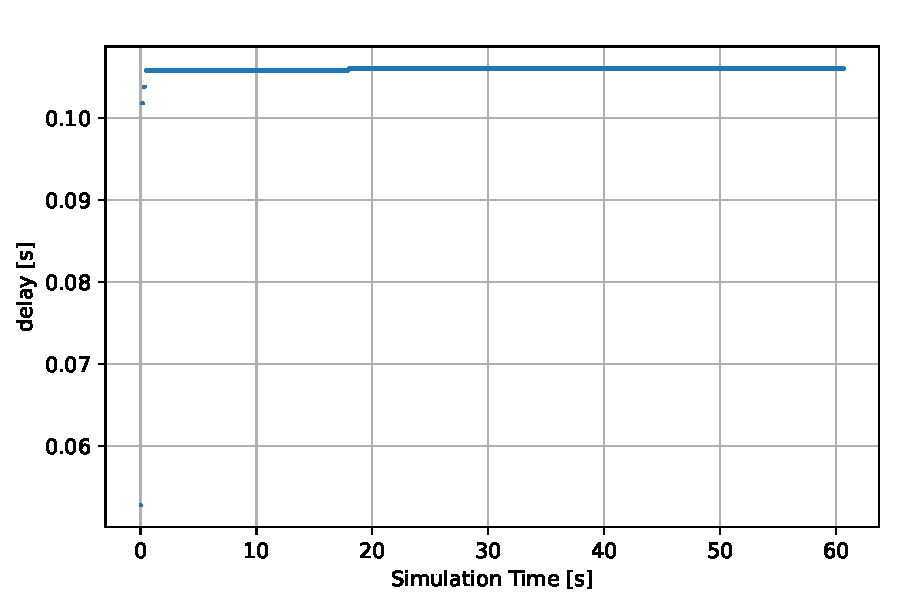
\includegraphics{graficas/WRR/delay_wrr.pdf}
    \caption{Retardo extremo a extremo WRR16}
    \label{fig:sinqos_pktreceived99100}
\end{figure}

\begin{figure}
    \centering
    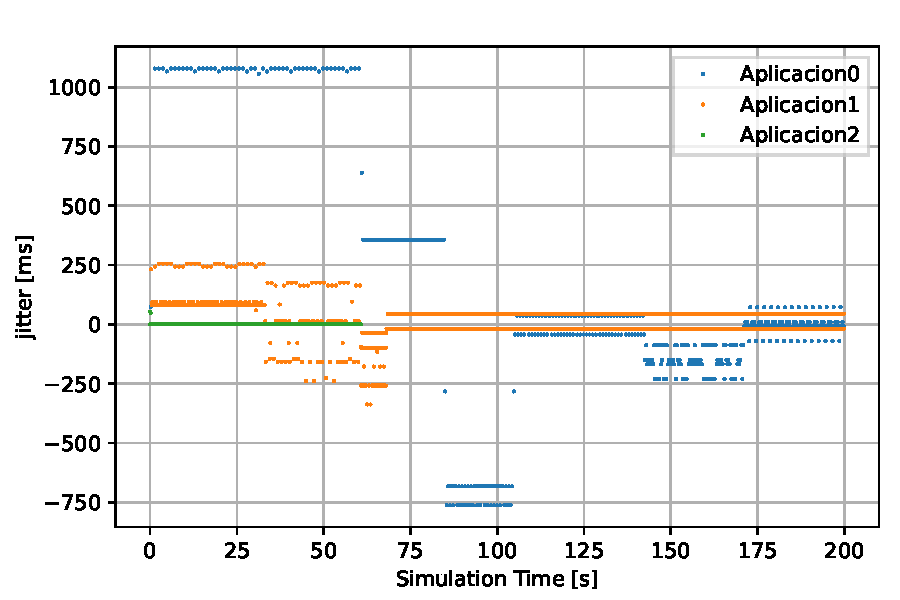
\includegraphics{graficas/WRR/jitter_WRR.pdf}
    \caption{Jitter a partir retardo extremo a extremo WRR16}
    \label{fig:sinqos_pktreceived99100}
\end{figure}

\begin{figure}
    \centering
    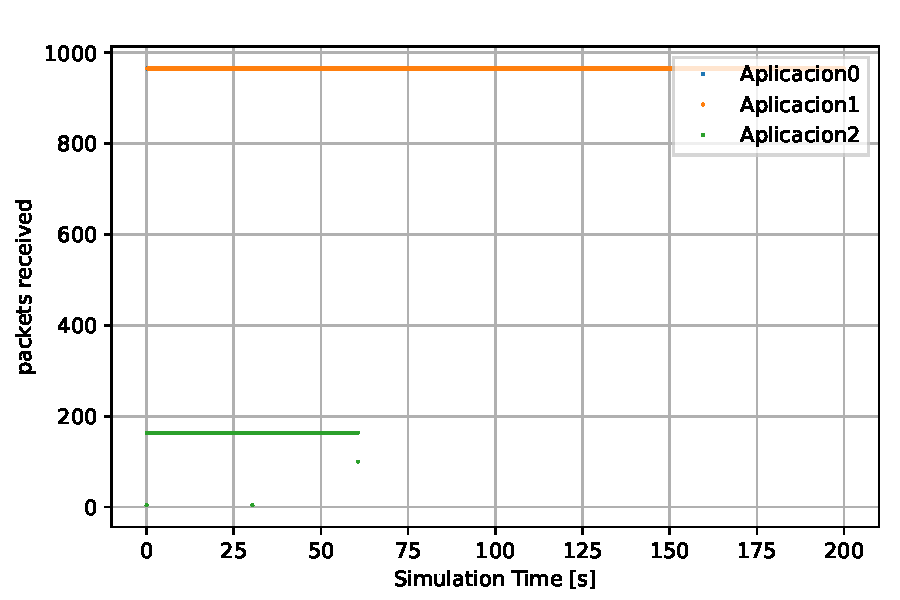
\includegraphics{graficas/WRR/packetsReceived_WRR.pdf}
    \caption{Paquetes recibidos en el servidor con WRR16}
    \label{fig:sinqos_pktreceived99100}
\end{figure}

\begin{figure}
    \centering
    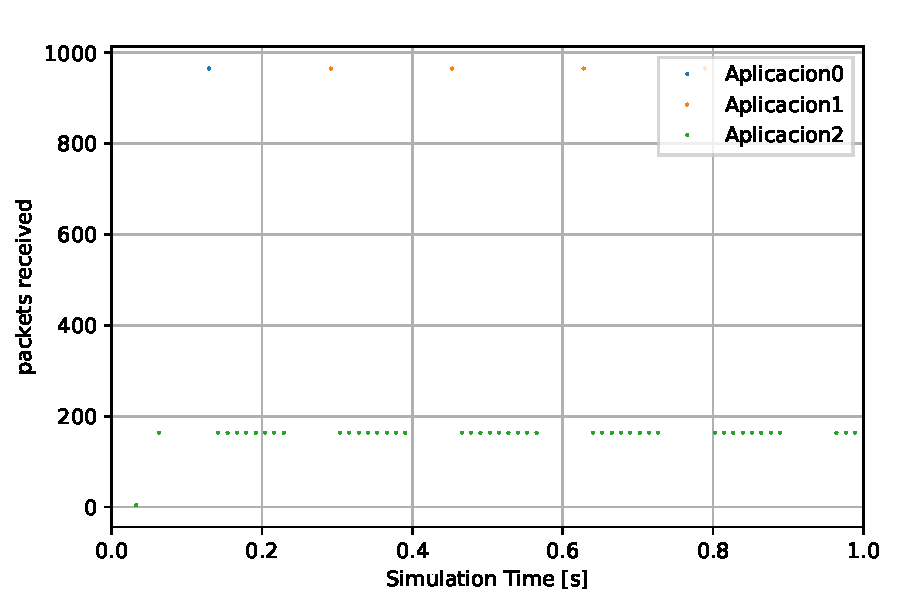
\includegraphics{graficas/WRR/packetsReceived_WRR_1.pdf}
    \caption{Paquetes recibidos en el servidor con WRR16 intervalo 0-1}
    \label{fig:sinqos_pktreceived99100}
\end{figure}

\begin{figure}
    \centering
    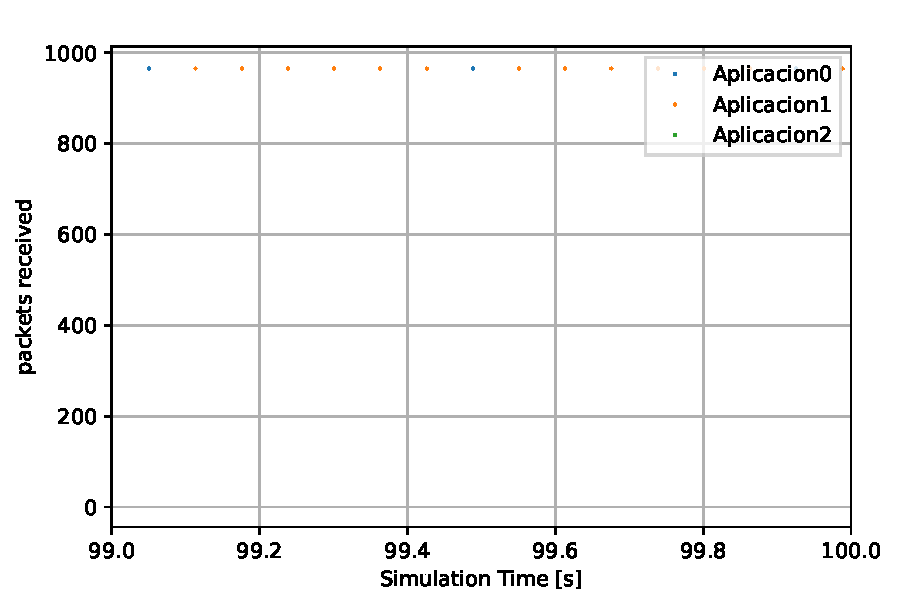
\includegraphics{graficas/WRR/packetsReceived_WRR_99.pdf}
    \caption{Paquetes recibidos en el servidor con WRR16 intervalo 99-100}
    \label{fig:sinqos_pktreceived99100}
\end{figure}

\begin{figure}
    \centering
    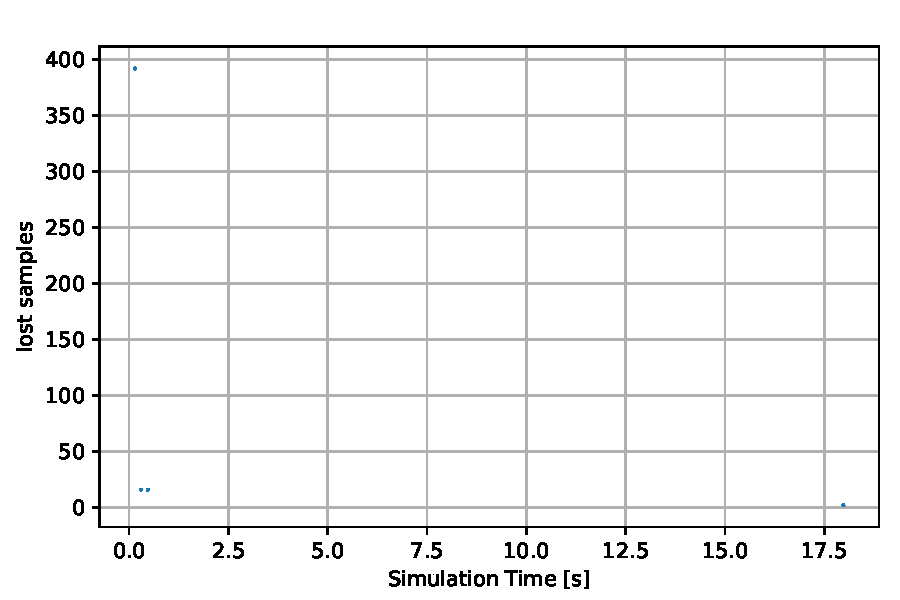
\includegraphics{graficas/WRR/muestras_perdidas_wrr.pdf}
    \caption{Muestras perdidas WRR16}
    \label{fig:sinqos_pktreceived99100}
\end{figure}


\begin{figure}[!ht]
    \centering
    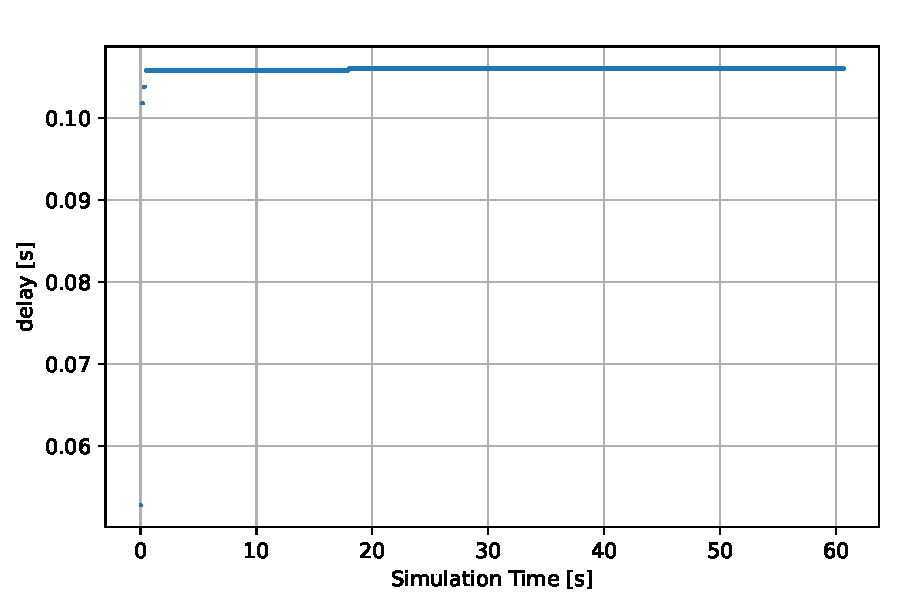
\includegraphics{graficas/RED/delay_red.pdf}
    \caption{Retardo extremo a extremo RED}
    \label{fig:sinqos_pktreceived99100}
\end{figure}

\begin{figure}
    \centering
    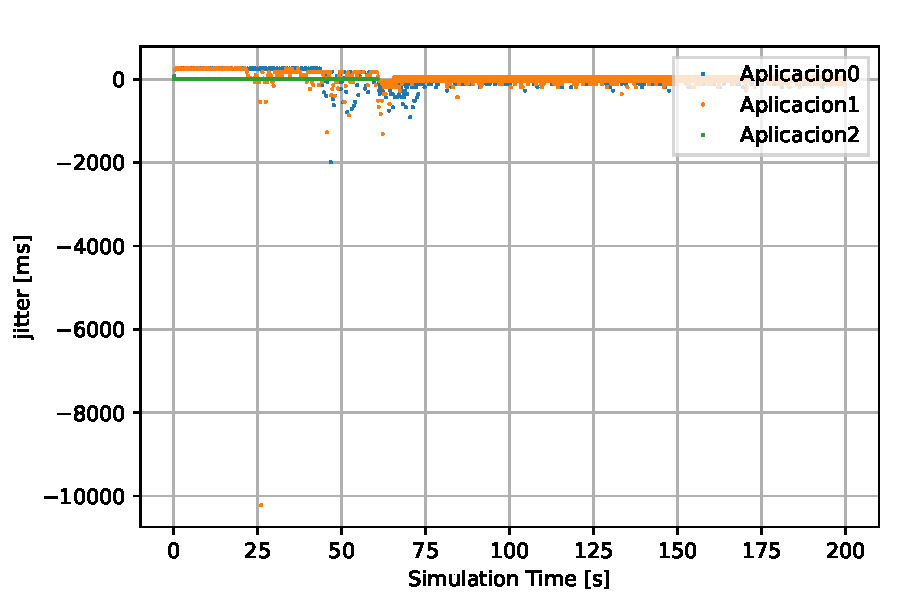
\includegraphics{graficas/RED/jitter_RED.pdf}
    \caption{Jitter a partir retardo extremo a extremo RED}
    \label{fig:sinqos_pktreceived99100}
\end{figure}

\begin{figure}
    \centering
    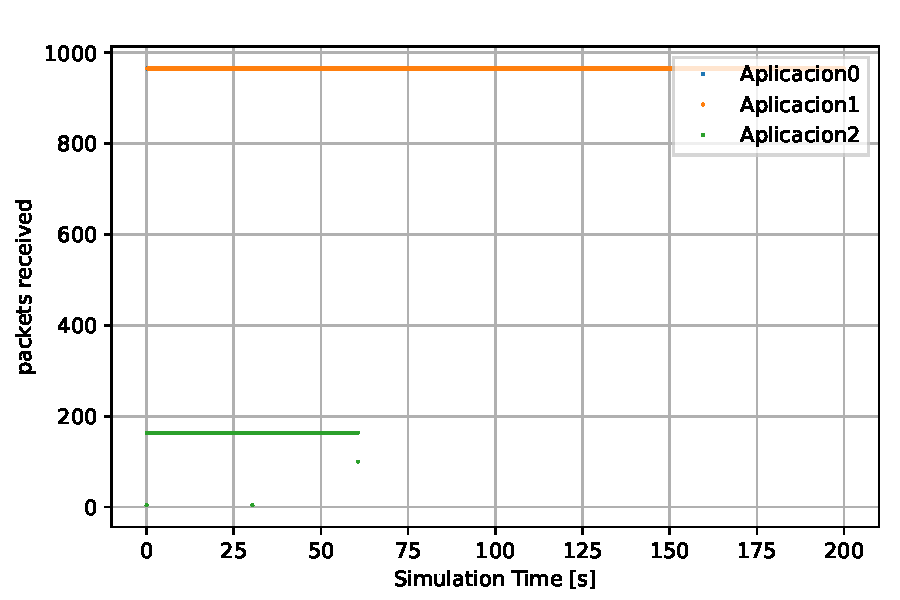
\includegraphics{graficas/RED/packetsReceived_RED.pdf}
    \caption{Paquetes recibidos en el servidor con RED}
    \label{fig:sinqos_pktreceived99100}
\end{figure}

\begin{figure}
    \centering
    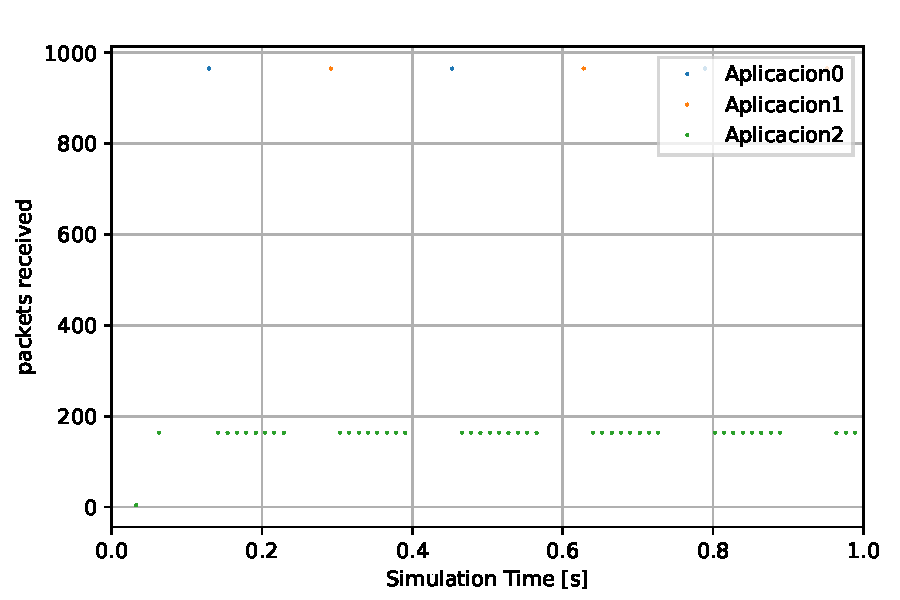
\includegraphics{graficas/RED/packetsReceived_RED_1.pdf}
    \caption{Paquetes recibidos en el servidor con RED intervalo 0-1}
    \label{fig:sinqos_pktreceived99100}
\end{figure}

\begin{figure}
    \centering
    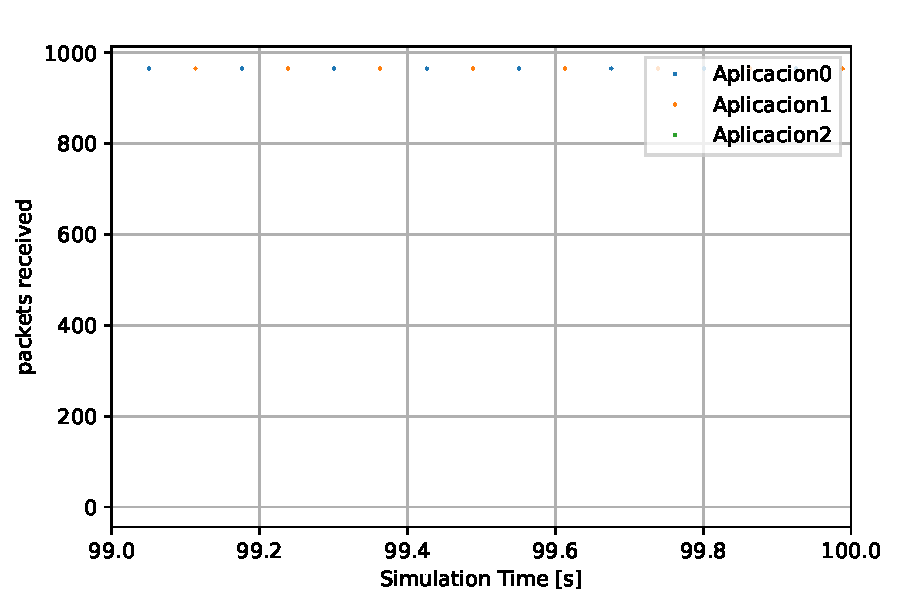
\includegraphics{graficas/RED/packetsReceived_RED_99.pdf}
    \caption{Paquetes recibidos en el servidor con RED intervalo 99-100}
    \label{fig:sinqos_pktreceived99100}
\end{figure}

\begin{figure}
    \centering
    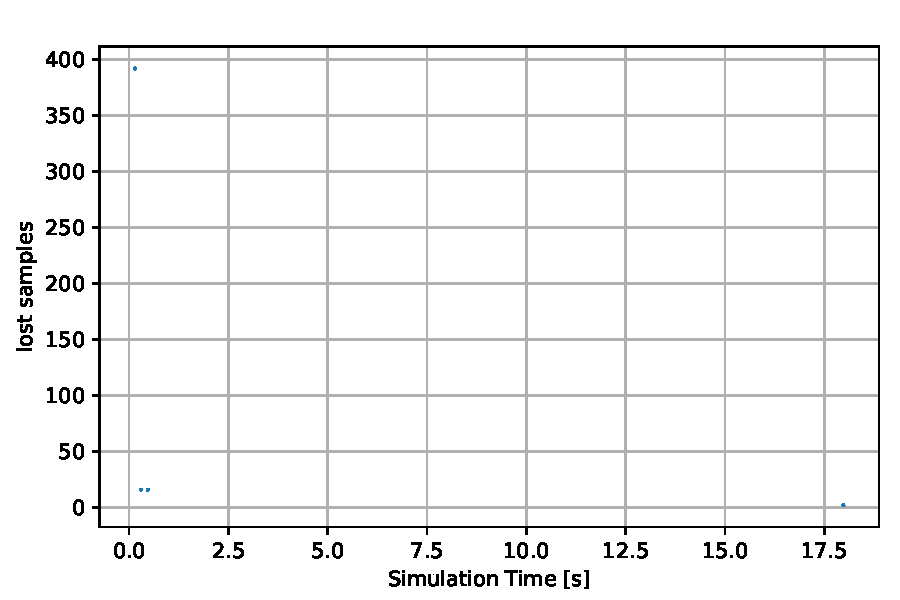
\includegraphics{graficas/RED/muestras_perdidas_red.pdf}
    \caption{Muestras perdidas con RED}
    \label{fig:sinqos_pktreceived99100}
\end{figure}




 %%%%%%%%%%%%%%%%%%%%%%%%%%%%%%%%%%%%%%%%
 % Apéndices, glosarios e bibliografía  %
 %%%%%%%%%%%%%%%%%%%%%%%%%%%%%%%%%%%%%%%%

%\appendix
%\appendixpage
%\chapter{Material adicional}
\label{chap:adicional}

\lettrine{E}{xemplo} de capítulo con formato de apéndice, onde se pode
incluír material adicional que non teña cabida no corpo principal do
documento, suxeito á limitación de 80 páxinas establecida no
regulamento de TFGs.

\Blindtext

%\include{anexos/...}

%\printglossary[type=\acronymtype,title=\nomeglosarioacronimos]
%\printglossary[title=\nomeglosariotermos]

%\bibliographystyle{IEEEtranN}
%\bibliography{\bibconfig,bibliografia/bibliografia}
%\clearpage
 
\end{document}

%%%%%%%%%%%%%%%%%%%%%%%%%%%%%%%%%%%%%%%%%%%%%%%%%%%%%%%%%%%%%%%%%%%%%%%%%%%%%%%%
